\RequirePackage{plautopatch}
\documentclass[13pt,aspectratio=169,xcolor=dvipsnames,table,dvipdfmx]{beamer}
\usepackage{bxdpx-beamer}

\usepackage{animate}
% \usepackage{svg}

\usepackage{adjustbox}      % \begin{adjustbox}
\usepackage[linesnumbered, ruled, vlined]{algorithm2e}    % \begin{algorithm2e}
\usepackage{amsmath}        % \begin{align*}
\usepackage{amssymb}        % \mathbb{A}
\usepackage{amsthm}         % \newtheorem
\usepackage{bm,bbm}         % \bm{A}, \bbm{1}
\usepackage{booktabs}       % \toprule, \midrule, \bottomrule
\usepackage{enumitem}       % \begin{enumerate}[label=(\alph*)]
\usepackage{hyperref}       % \href{URL}{text}
\usepackage{ifthen}         % \ifthenelse
\usepackage{lipsum}         % \lipsum
\usepackage{makecell}       % \makecell{L1\L2}
\usepackage{mathrsfs}       % \mathscr{A}
\usepackage{mathtools}      % \mathrlap
\usepackage{multirow}       % \multirow
\usepackage[authoryear]{natbib}
\usepackage{optidef}        % \begin{mini*}{x}{f(x)}{}{}
\usepackage{orcidlink}      % \orcidlink
\usepackage{physics}        % \qty, \norm, \abs
\usepackage{subcaption}     % \captionsetup
\usepackage{subfiles}       % \subfile{file}
\usepackage{thm-restate}    % \begin{restatable}{theorem}{thm}
\usepackage{tikz}           % \begin{tikzpicture}
\usepackage{xparse}         % \NewDocumentCommand

\definecolor{cA}{HTML}{0072BD}
\definecolor{cB}{HTML}{EDB120}
\definecolor{cC}{HTML}{77AC30}
\definecolor{cD}{HTML}{D95319}

\newcommand{\red}[1]{\textcolor{red}{#1}}
\newcommand{\blue}[1]{\textcolor{blue}{#1}}
\newcommand{\cyan}[1]{\textcolor{cyan}{#1}}
\newcommand{\gray}[1]{\textcolor{gray}{#1}}
\newcommand{\green}[1]{\textcolor{green}{#1}}
\newcommand{\brown}[1]{\textcolor{brown}{#1}}
\newcommand{\black}[1]{\textcolor{black}{#1}}
\newcommand{\orange}[1]{\textcolor{orange}{#1}}
\newcommand{\purple}[1]{\textcolor{purple}{#1}}
\newcommand{\tccA}[1]{\textcolor{cA}{#1}}
\newcommand{\tccB}[1]{\textcolor{cB}{#1}}
\newcommand{\tccC}[1]{\textcolor{cC}{#1}}
\newcommand{\tccD}[1]{\textcolor{cD}{#1}}
\newcommand{\st}{\text{ s.t. }}
\newcommand{\Img}[1]{\mathrm{Im}\qty(#1)}
\newcommand{\Ker}[1]{\mathrm{Ker}\qty(#1)}
\newcommand{\Supp}[1]{\mathrm{supp}\qty(#1)}
\newcommand{\Rank}[1]{\mathrm{rank}\qty(#1)}
\newcommand{\floor}[1]{\left\lfloor #1 \right\rfloor}
\newcommand{\ceil}[1]{\left\lceil #1 \right\rceil}
% C++ (https://tex.stackexchange.com/questions/4302/prettiest-way-to-typeset-c-cplusplus)
\newcommand{\Cpp}{C\nolinebreak[4]\hspace{-.05em}\raisebox{.4ex}{\relsize{-3}{\textbf{++}}}}
% https://tex.stackexchange.com/questions/28836/typesetting-the-define-equals-symbol
\newcommand{\defeq}{\coloneqq}
\newcommand{\eqdef}{\eqqcolon}
% https://tex.stackexchange.com/questions/5502/how-to-get-a-mid-binary-relation-that-grows
\newcommand{\relmiddle}[1]{\mathrel{}\middle#1\mathrel{}}

% https://tex.stackexchange.com/questions/564216/newcommand-for-each-letter
\ExplSyntaxOn
\NewDocumentCommand{\definealphabet}{mmmm}{
\int_step_inline:nnn{`#3}{`#4}{
\cs_new_protected:cpx{#1 \char_generate:nn{##1}{11}}{
\exp_not:N #2{\char_generate:nn{##1}{11}}}}}
\ExplSyntaxOff

\definealphabet{bb}{\mathbb}{A}{Z}
\definealphabet{rm}{\mathrm}{A}{Z}
\definealphabet{cal}{\mathcal}{A}{Z}
\definealphabet{frak}{\mathfrak}{a}{z}
% \definealphabet{scr}{\mathscr}{A}{Z}
% \definealphabet{frak}{\mathfrak}{A}{Z}

% https://qiita.com/rityo_masu/items/efd44bc8f9229e014237
\allowdisplaybreaks[4]

\usetikzlibrary{
  3d,
  % fit,
  calc,
  math,
  matrix,
  patterns,
  backgrounds,
  arrows.meta,
  shapes.geometric,
  decorations.pathmorphing,
}

% === Beamer Settings ===

% https://uplatexmemo.hatenadiary.jp/entry/2021/01/04/130013
\usepackage{caption}
\captionsetup[figure]{justification=centering}

%Beamerの設定
\usetheme{Boadilla}

%Beamerフォント設定
\usefonttheme{professionalfonts} % Be professional!
\usepackage[T1]{fontenc}
\usepackage{mlmodern}  % 太いComputer Modern
% MLmodernのバグを修正: cf. https://tex.stackexchange.com/questions/646333/size-of-integral-symbol-in-section-header-with-mlmodern
\DeclareFontFamily{OMX}{mlmex}{}
\DeclareFontShape{OMX}{mlmex}{m}{n}{%
   <->mlmex10%
   }{}
\usepackage{newtxtext} % 数式以外をTXフォントで上書き
\usepackage[deluxe,uplatex]{otf} % 日本語多ウェイト化
\renewcommand{\familydefault}{\sfdefault}  % 英文をサンセリフ体に
\renewcommand{\kanjifamilydefault}{\gtdefault}  % 日本語をゴシック体に
\usefonttheme{structurebold} % タイトル部を太字
\setbeamerfont{alerted text}{series=\bfseries} % Alertを太字
\setbeamerfont{section in toc}{series=\mdseries} % 目次は太字にしない
\setbeamerfont{frametitle}{size=\Large} % フレームタイトル文字サイズ

\usefonttheme{structurebold}
\useinnertheme{circles}
\setbeamerfont{alerted text}{series=\bfseries}
\setbeamerfont{section in toc}{series=\mdseries}
\setbeamerfont{itemize/enumerate body}{size=\large}
\setbeamertemplate{blocks}[rounded]
\setbeamertemplate{footline}[frame number]
\setbeamertemplate{navigation symbols}{} % ナビゲーションシンボルを消す
\setbeamertemplate{title page}{%
\centering
    \vspace{2.5em}
    {\usebeamerfont{title} \usebeamercolor[fg]{title} \inserttitle \par}
    {\usebeamerfont{subtitle}\usebeamercolor[fg]{subtitle} \insertsubtitle \par}
    \vspace{3.0em}
    \usebeamerfont{author}\insertauthor\par
    \usebeamerfont{institute}\insertinstitute \par
    \vspace{1.5em}
    \usebeamerfont{date}\insertdate\par
    \usebeamercolor[fg]{titlegraphic}\inserttitlegraphic
}

%Beamer Color
\definecolor{blendedblue}{rgb}{0.2,0.2,0.7}
\definecolor{UniBlue}{RGB}{0,150,200}
\definecolor{UniGreen}{RGB}{0,200,150}
\definecolor{AlertOrange}{RGB}{255,76,0}
\definecolor{AlmostBlack}{RGB}{38,38,38}
\setbeamercolor{normal text}{fg=AlmostBlack}
\setbeamercolor{structure}{fg=UniGreen}
\setbeamercolor{block title}{fg=UniGreen!50!black}
\setbeamercolor{alerted text}{fg=AlertOrange}
\setbeamercolor{itemize item}{fg=black}
\setbeamercolor{itemize subitem}{fg=black}
\setbeamercolor{itemize subsubitem}{fg=black}

\hypersetup{colorlinks=true,linkcolor=UniGreen,citecolor=blue,urlcolor=blue}

\setbeamerfont{section in toc}{size=\LARGE}
\AtBeginSection[]{
    \frame{\tableofcontents[currentsection, hideallsubsections]}
}

% === TITLE ===
\title{\huge{最適化手法を用いた\\グラフ描画とその初期配置}}
\author{\Large{\textbf{浜口 広樹}, 丸茂直貴, 武田朗子}}
\institute{\large{東京大学 大学院 情報理工学系研究科}}
\date{2025/5/31}

\newif\ifShowHidden
% \ShowHiddenfalse
\ShowHiddentrue

\begin{document}

\ifShowHidden
  \maketitle
\fi

\ifShowHidden
  \begin{frame}{グラフ描画とは}
    \begin{columns}
      \begin{column}{0.6\columnwidth}
        \large{%
          グラフ $G = (V,E)$ (頂点集合 $V$  / 辺集合 $E$)\\
          \textbf{グラフ描画}\normalsize{は視覚化における重要なタスクの一つ}\\
          \textbf{力学モデル (特に、FRモデル)}\normalsize{に基づく描画手法が有名}\\
        }
        \vspace{1em}
        \begin{figure}[htbp]
          \centering
          \begin{minipage}{0.52\columnwidth}
            \centering
            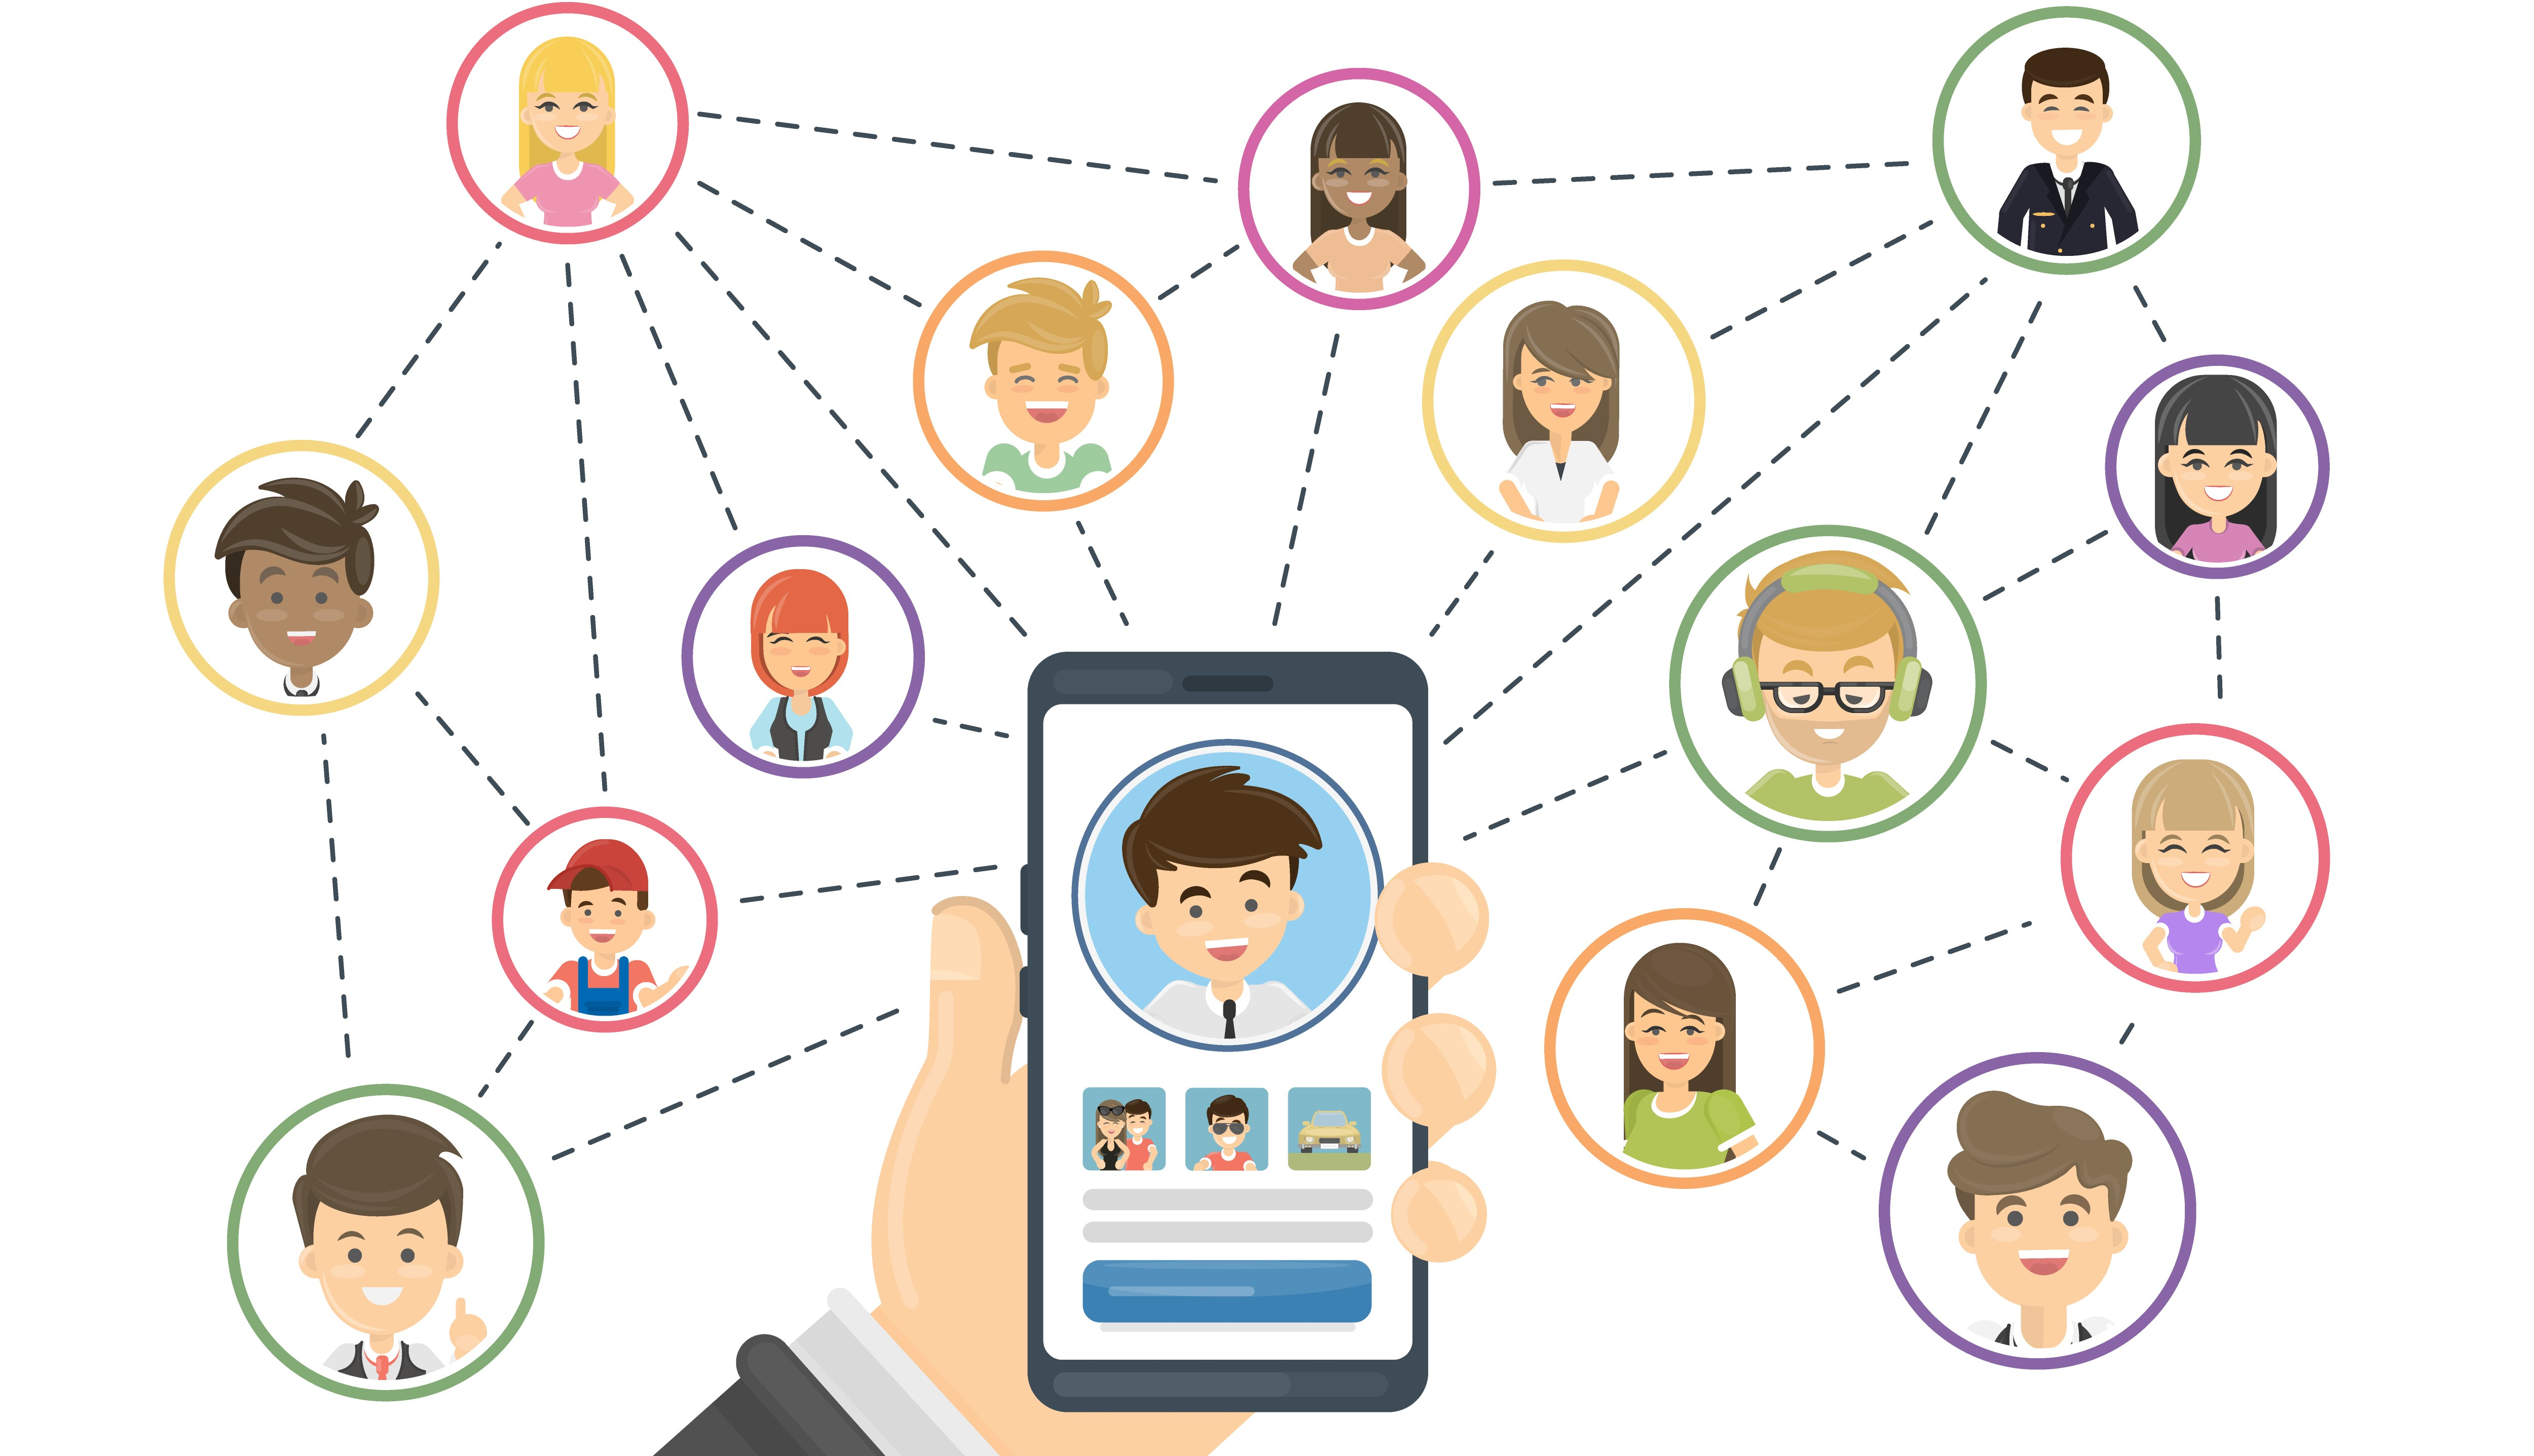
\includegraphics[width=\columnwidth]{introExample/social.jpg}
            \caption*{
              SNSのフォロー関係\\
              を表すグラフ\\
              \gray{\footnotesize{Designed~by~\href{www.freepik.com}{Freepik}}}
            }
          \end{minipage}%
          \begin{minipage}{0.48\columnwidth}
            \centering
            
\includegraphics[width=\columnwidth]{introExample/knowledge.png}
            \caption*{
              関連性を表す知識グラフ\\
              Google Knowledge Graphや\\
              Obsidian(ノートエディタ)\\
              \gray{\footnotesize{By~\href{https://realkm.com/2023/06/12/introduction-to-knowledge-graphs-section-5-1-inductive-knowledge-graph-analytics/}{RealKM}}}
            }
          \end{minipage}%
        \end{figure}
      \end{column}
      \begin{column}{0.4\columnwidth}
        \centering
        \vspace{-1.5em}
        \begin{figure}[htbp]
          \centering
          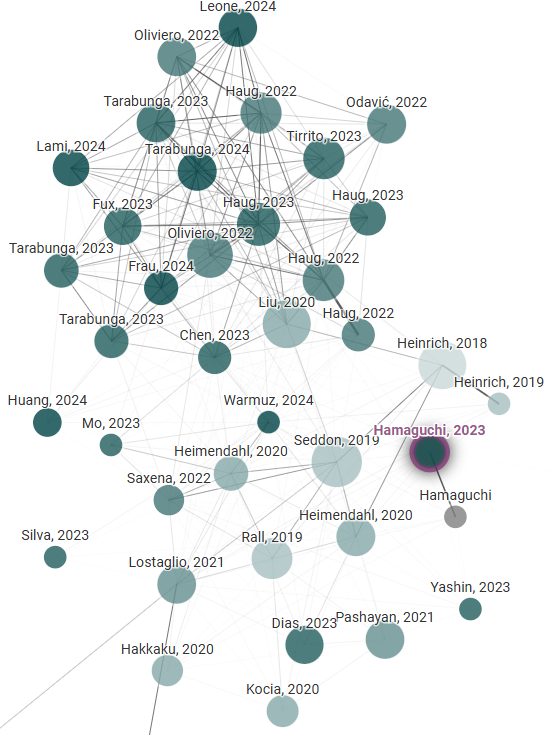
\includegraphics[height=0.77\textheight]{introExample/connectedPapers.png}
          \caption*{
            論文の引用関係を表すグラフ\\
            \gray{\footnotesize{By~\raisebox{-0.4\baselineskip}{
\includegraphics[height=0.07\textheight]{introExample/connectedPapersLogo.png}}
                (\href{https://www.connectedpapers.com/}{Link})}
            }}
        \end{figure}
      \end{column}
    \end{columns}
  \end{frame}
\fi

\ifShowHidden
  \begin{frame}{Fruchterman--Reingold力学モデル}
    \tccA{\Large{\textbf{a}}}\tccA{ttractive force (引力)}と
    \tccD{\Large{\textbf{r}}}\tccD{epulsive force (斥力)}が働く \citep{fruchtermanGraphDrawingForcedirected1991}
    \begin{equation*}
      \tccA{F_{i,j}^\mathrm{a}(d) \defeq \frac{w_{i,j} d^2}{k}}, \quad \tccD{F^\mathrm{r}(d) \defeq -\frac{k^2}{d}}.
    \end{equation*}
    \textbf{力指向グラフ描画}はこれらの力の\textbf{均衡点}を単純なシミュレーションで求める。\\
    \textbf{Multilevel Approach}という複雑だが強力な手法も併用可能 (GraphVizなど)~\citep{Hu2006EfficientHF}
    \begin{columns}
      \begin{column}{0.5\columnwidth}
        \begin{figure}[h]
          \centering
          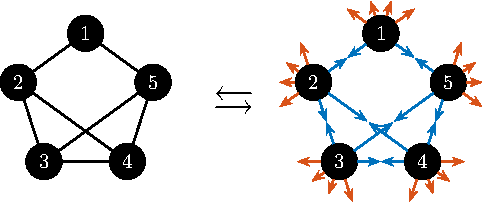
\includegraphics[width=\columnwidth]{../main/fr_layout/fr_layout1.pdf}
          \caption*{\large{$w_{i,j} > 0 \iff \{i,j\} \in E$}}
        \end{figure}
      \end{column}
      \begin{column}{0.5\columnwidth}
        \begin{figure}[h]
          \centering
          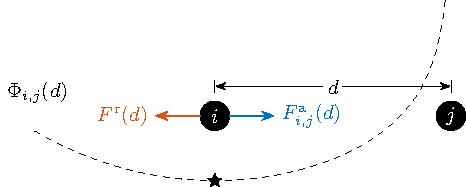
\includegraphics[width=\columnwidth]{../main/fr_layout/fr_layout2.pdf}
          \caption*{\large{$d = \norm{x_i - x_j}$}}
        \end{figure}
      \end{column}
    \end{columns}
  \end{frame}
\fi


\ifShowHidden
  \begin{frame}{NetworkXによるグラフ描画}
    \begin{columns}
      \begin{column}{0.62\columnwidth}
        \large{%
          \textbf{NetworkX} \raisebox{-0.4\baselineskip}{
\includegraphics[width=2em]{graphDrawing/networkxLogo.png}} は著名なPythonライブラリ\\
          \texttt{nx.draw}: \large{\textbf{FR}}力学モデルを用いたグラフ描画
        }
        \begin{center}
          \rule{0.8\columnwidth}{0.4pt}
        \end{center}
        \Large{
          \uncover<1->{$\abs{V}=\phantom{0}10$: \phantom{1}0.2 sec / 完璧な円形を描画}\\
          \uncover<2->{$\abs{V}=\phantom{0}20$: \phantom{1}0.2 sec / 捻じれが生じ出す}\\
          \uncover<3->{$\abs{V}=500$: \red{11.5} sec / \red{壊滅的な描画結果}}
        }
      \end{column}
      \begin{column}{0.38\columnwidth}
        \begin{figure}[htbp]
          \centering
          \only<1>{
\includegraphics[width=\columnwidth]{vscode/10.png}}%
          \only<2>{
\includegraphics[width=\columnwidth]{vscode/20.png}}%
          \only<3>{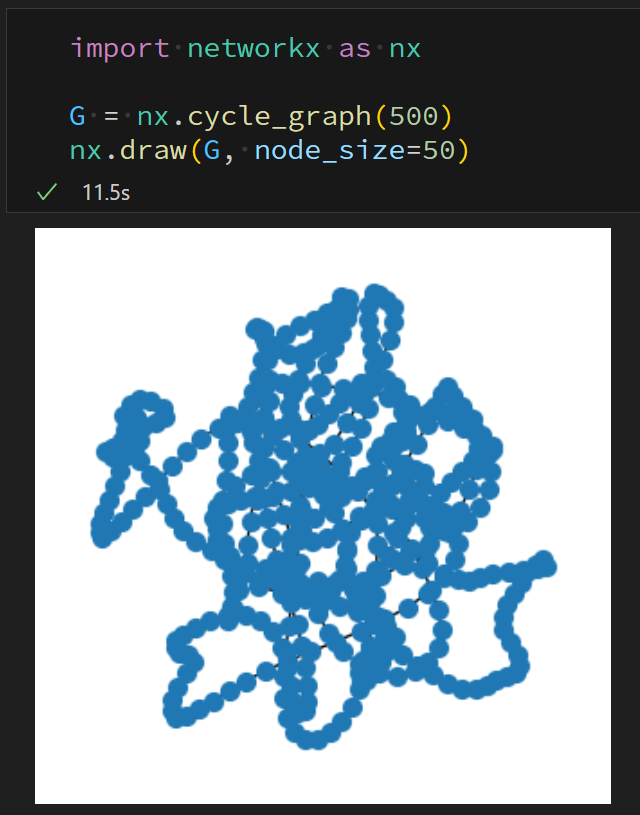
\includegraphics[width=\columnwidth]{vscode/500.png}}%
        \end{figure}
      \end{column}
    \end{columns}
  \end{frame}
\fi

\ifShowHidden
  \begin{frame}{``捻じれ'' がもたらす停滞}
    \large{%
      \textbf{捻じれ}とは、不必要な辺の交差や歪んだグラフ構造を指す。\\
      \citep{veldhuizenDynamicMultilevelGraph2007,cheongSnapshotVisualizationComplex2018}\\
      $\to$ 特に中大規模なグラフ描画において、深刻な問題となる。\\
      \textbf{これを\red{2つの数理最適化手法によるアプローチ}で解決するのが本研究の目的。}\\
    }
    \begin{figure}[htbp]
      \centering
      \animategraphics[autoplay,loop,width=0.38\columnwidth]{5}{circle/circle-}{1}{1}%!!!50
    \end{figure}
  \end{frame}
\fi

\ifShowHidden
  \begin{frame}{問題の定式化}
    \begin{columns}
      \begin{column}{0.7\columnwidth}
        従来的解釈: \tccA{引力}と\tccD{斥力}の均衡点を求めてグラフ描画\\
        \begin{equation*}
          \tccA{F_{i,j}^\mathrm{a}(d) \defeq \frac{w_{i,j} d^2}{k}}, \quad \tccD{F^\mathrm{r}(d) \defeq -\frac{k^2}{d}}.
        \end{equation*}
      \end{column}
      \begin{column}{0.3\columnwidth}
        \vspace{-2.5em}
        \begin{figure}[h]
          \centering
          
\includegraphics[width=\columnwidth]{../main/energy_3d/energy_3d.png}
        \end{figure}
      \end{column}
    \end{columns}
    これらのスカラーポテンシャル (エネルギー) は次のように定義される~\citep{6183577}。
    \begin{gather*}
      \tccA{E_{i,j}^\mathrm{a}(d) \defeq \int_{0}^{d} F_{i,j}^\mathrm{a}(r) \dd{r} = \frac{w_{i,j} d^3}{3k}}, \quad
      \tccD{E^\mathrm{r}(d)       \defeq \int_{\infty}^{d} F^\mathrm{r}(r) \dd{r} = -k^2\log{d}}, \\
      E_{i,j}(d)            \defeq \tccA{E_{i,j}^\mathrm{a}(d)} + \tccD{E^\mathrm{r}(d)}.
    \end{gather*}
    均衡点を求める $\iff$ \textbf{$f(X)$ の局所最適解を求める} (\textbf{非凸最適化問題})
    \begin{mini*}
      {X \in \bbR^{2 \times n}}
      {f(X) \defeq \sum_{i<j} E_{i,j}(\norm{x_i - x_j}).}
      {}
      {}
    \end{mini*}
  \end{frame}
\fi

\ifShowHidden
  \begin{frame}{貢献1: L-BFGS法による最適化 (NetworkXに実装を提案)}
    \begin{columns}
      \begin{column}{0.3\columnwidth}
        \textbf{L-BFGS法}を用いる\\
        無制約問題に対する\mbox{微分}\mbox{情報}を用いた最適化手法\\[0.5em]

        効率的と知られていた。\citep{6183577}\\[0.5em]

        \textbf{主に実装面での貢献}\\
        軽量な実装が特徴\\
        (NetworkXというOSSで\\次バージョンより採用予定)\\[0.5em]

        次ページで述べる非有界な場合に対する\textbf{モデル修正}\\などを新規に提案した。
      \end{column}%
      \begin{column}{0.7\columnwidth}
        \begin{figure}[h]
          \centering
          
\includegraphics[width=\columnwidth]{imgs/tsukuba1.png}
        \end{figure}
      \end{column}
    \end{columns}
  \end{frame}
\fi

\ifShowHidden
  \begin{frame}{貢献1: L-BFGS法による最適化 (非有界に対処するモデル修正)}
    \begin{columns}
      \begin{column}{0.3\columnwidth}
        力学に基づくシミュレーションは、
        非連結グラフや負辺ありでも動く。\\[0.5em]

        しかし、最適化問題としては
        実は\textbf{非有界}となる。\\[0.5em]

        \red{不合理な描画結果に!}\\[0.5em]

        連結グラフの場合に対する\\
        理論的同一性を保ちながら\\
        重なりが生じにくい\textbf{重力項}\\
        を導入した。
      \end{column}%
      \begin{column}{0.7\columnwidth}
        \begin{figure}[h]
          \centering
          
\includegraphics[width=\columnwidth]{imgs/tsukuba2.png}
        \end{figure}
      \end{column}
    \end{columns}
  \end{frame}
\fi

\ifShowHidden
  \begin{frame}{貢献2: 座標ニュートン方向を用いた初期配置}
    \textbf{\red{数理最適化によるアプローチを更に高速化出来ないか? $\to$ 初期配置(2つ目の貢献)}}\\
    \textbf{焼き鈍し法}~\citep{ghassemitoosiSimulatedAnnealingPreProcessing2016}よりも、より広く適用出来る方法を提案。
    \begin{figure}[h]
      \centering
      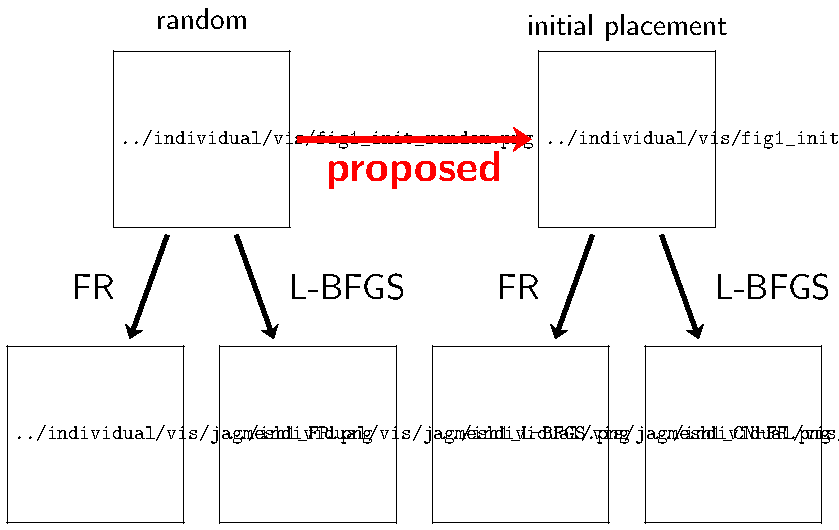
\includegraphics[width=0.7\columnwidth]{../main/fig1/fig1_slide.pdf}
    \end{figure}
  \end{frame}
\fi

\ifShowHidden
  \begin{frame}{貢献2: 問題の簡略化 (1/2)}
    \textbf{初期配置として大まかな解を高速に得たい。} \quad
    元問題の代わりに次を解く:
    \begin{columns}
      \begin{column}{0.55\columnwidth}
        \begin{mini}
          {X \in \bbR^{2 \times n}}
          {\sum_{\{i,j\}\in E} \frac{w_{i,j}\norm{x_i - x_j}^3}{3k},}
          {\label{eq:frApprox0}}
          {}
          \addConstraint{x_i}{\in Q^\mathrm{hex} \quad}{\text{for $1 \leq i \leq n$}}
          \addConstraint{x_i}{\neq x_j \quad}{\text{for $1 \leq i < j \leq n$}.}
        \end{mini}
        where
        \begin{equation*}
          Q^\mathrm{hex} \defeq \left\{ \qty(q+\tfrac{1}{2}r, \tfrac{\sqrt{3}}{2}r) \relmiddle| q \in \bbZ, r \in \bbZ \right\}.
        \end{equation*}
      \end{column}
      \begin{column}{0.45\columnwidth}
        \begin{figure}[t]
          \centering
          
\includegraphics[width=\columnwidth]{../main/pi/pi.pdf}
        \end{figure}
      \end{column}
    \end{columns}
    \vspace{0.3cm}
    \hrulefill\\
    この導出理由: 元問題 $\text{minimize} \ f(X)$ において
    まず $f(X)$ を $\tccA{E^\mathrm{a}_{i,j}}$ と $\tccD{E^\mathrm{r}}$ に分離する
    \begin{mini*}
      {X \in \bbR^{2 \times n}}
      {\tccA{\sum_{\{i,j\}\in E} \frac{w_{i,j}\norm{x_i - x_j}^3}{3k}} - \tccD{\sum_{i<j} k^2\log{\norm{x_i - x_j}}}.}
      {}
      {}
    \end{mini*}
  \end{frame}
\fi

\ifShowHidden
  \begin{frame}{貢献2: 問題の簡略化 (2/2)}
    先行研究~\citep{ghassemitoosiSimulatedAnnealingPreProcessing2016}に従い、$x_i$の位置を離散点集合$Q$に固定する:
    \begin{mini*}
      {X \in \bbR^{2 \times n}}
      {\tccA{\sum_{\{i,j\}\in E} \frac{w_{i,j}\norm{x_i - x_j}^3}{3k}} - \tccD{\sum_{i<j} k^2\log{\norm{x_i - x_j}}},}
      {}
      {}
      \addConstraint{x_i}{\in Q \quad}{\text{for $1 \leq i \leq n$}}
      \addConstraint{x_i}{\neq x_j \quad}{\text{for $1 \leq i < j \leq n$}.}
    \end{mini*}
    $\tccA{\abs{\{\{i,j\} \st \{i,j\} \in E\}} = \abs{E}} \ll \tccD{\abs{\{\{i,j\} \st i<j\}} = \order{\abs{V}^2}}$. 第二項を落としたい。\\
    $\norm{q_i - q_j} \geq \epsilon$ $(q_i,q_j \in Q, q_i \neq q_j)$ を満たす $Q$ を取ると、第二項の影響を抑えられる。
    \begin{mini*}
      {X \in \bbR^{2 \times n}}
      {\tccA{f^\mathrm{a}(X) \defeq \sum_{\{i,j\}\in E} \frac{w_{i,j}\norm{x_i - x_j}^3}{3k}},}
      {\label{eq:frApprox2}}
      {}
      \addConstraint{\tccD{x_i}}{\tccD{\in Q \quad}}{\text{for $1 \leq i \leq n$}}
      \addConstraint{\tccD{x_i}}{\tccD{\neq x_j \quad}}{\text{for $1 \leq i < j \leq n$}.}
    \end{mini*}
    $Q$としては六方最密構造を用いる。
  \end{frame}
\fi

% \ifShowHidden
\begin{frame}{貢献2: ここまでのまとめ}
  元々の問題は以下であった:
  \begin{mini*}
    {X \in \bbR^{2 \times n}}
    {f(X) \defeq \sum_{i<j} E_{i,j}(\norm{x_i - x_j}) = \tccA{\sum_{\{i,j\}\in E} \frac{w_{i,j}\norm{x_i - x_j}^3}{3k}} - \tccD{\sum_{i<j} k^2\log{\norm{x_i - x_j}}}.}
    {}
    {}
  \end{mini*}
  \begin{columns}
    \begin{column}{0.55\columnwidth}
      次のように簡略化すること高速化を図る:
      \begin{mini*}
        {X \in \bbR^{2 \times n}}
        {\tccA{f^\mathrm{a}(X) \defeq \sum_{\{i,j\}\in E} \frac{w_{i,j}\norm{x_i - x_j}^3}{3k}}}
        {}
        {}
        \addConstraint{\tccD{x_i}}{\tccD{\in Q^\mathrm{hex} \quad}}{\text{for $1 \leq i \leq n$}}
        \addConstraint{\tccD{x_i}}{\tccD{\neq x_j \quad}}{\text{for $1 \leq i < j \leq n$}.}
      \end{mini*}
    \end{column}
    \begin{column}{0.45\columnwidth}
      \begin{figure}[t]
        \centering
        
\includegraphics[width=\columnwidth]{../main/pi/pi.pdf}
      \end{figure}
    \end{column}
  \end{columns}
  次以降で簡略化後の問題を解く方法を説明する。
\end{frame}
% \fi

% \ifShowHidden
\begin{frame}{貢献2: 提案アルゴリズムの基礎 -- 確率的座標降下法}
  $f\colon \bbR^n \to \bbR$ を狭義凸関数とする。$x_0$ における2次近似は次のように表される:
  \begin{equation*}
    f(x) \approx f(x_0) + \nabla f(x_0)^\top (x - x_0) + \frac{1}{2} (x - x_0)^\top \nabla^2 f(x_0) (x - x_0).
  \end{equation*}
  最小値 $x^*$ は次を満たす:
  \begin{align*}
         & \nabla f(x_0) + \nabla^2 f(x_0) (x^* - x_0) = 0                                              \\
    \iff & x^* = x_0 \red{- \nabla^2 f(x_0)^{-1} \nabla f(x_0)}. \qquad \text{\textbf{\red{(ニュートン方向)}}}
  \end{align*}
  これは優れた更新則だが、ニュートン方向の計算は\textbf{非常に高コスト}...\\[1em]

  我々は \large{\textbf{確率的座標降下法}} を \large{\textbf{\red{座標ニュートン方向}}} と組み合わせて使用する。\\
  $f_i(x_i)$ を $i$ 番目の座標（ランダムに選択）に制限した関数とする。\\
  座標ニュートン方向: $d_i = -\nabla^2 f_i(x_i)^{-1} \nabla f_i(x_i)$ \red{$\leftarrow$ \large{\textbf{低コスト！計算可能！}}}
\end{frame}
% \fi

% \ifShowHidden
% \begin{frame}{貢献2: 提案アルゴリズム (1/2) -- 座標ニュートン方向}
%   問題~\eqref{eq:frApprox0} を\textbf{座標ニュートン方向}を用いて解く \quad
%   頂点 $v_i$ に対応する $f^{\mathrm{a}}_i(x_i)$ を
%   \begin{equation*}
%     f^{\mathrm{a}}_i(x_i) \defeq \sum_{j \neq i} \frac{w_{i,j}\norm{x_i - x_j}^3}{3k}
%   \end{equation*}
%   と定める。
%   その勾配とヘッセ行列は
%   \begin{align*}
%     \nabla f^{\mathrm{a}}_i(x_i)   & = \sum_{j \neq i} \frac{w_{i,j}\norm{x_i - x_j}}{k} (x_i - x_j),                                                                                                                      \\
%     \nabla^2 f^{\mathrm{a}}_i(x_i) & = \sum_{j \neq i} \frac{w_{i,j}\norm{x_i - x_j}}{k} \begin{pmatrix}1 & 0 \\[0.3em]0 & 1\end{pmatrix} + \sum_{j \neq i} \frac{w_{i,j}}{k\norm{x_i - x_j}} (x_i - x_j)(x_i - x_j)^\top.
%   \end{align*}
%   $f^{\mathrm{a}}_i$ は \textbf{凸}で、
%   問題\eqref{eq:fr} の $E_{i,j}(\norm{\cdot - x_j})$ や ~\eqref{eq:frApprox0} の $f^{\mathrm{a}}(\cdot)$ (非凸) とは異なる\\
%   座標制限による恩恵の一つ
% \end{frame}
% \fi

% \ifShowHidden
\begin{frame}{貢献2: 提案アルゴリズム -- 更新則}
  $f^{\mathrm{a}}_i$に限定すると\textbf{凸関数になる}ことに注意する。\quad
  通常の更新則:
  \begin{equation*}
    x_i^\mathrm{new} \gets x_i - \nabla^2 f^{\mathrm{a}}_i(x_i)^{-1} \nabla f^{\mathrm{a}}_i(x_i).
  \end{equation*}
  $x_i^\mathrm{new}$ は六角格子 $Q^\mathrm{hex}$ に含まれるとは限らず、
  $Q^\mathrm{hex}$ 上の最近点に丸める必要がある。\\
  経験的に、ランダムノイズを加えることが効果的である(焼き鈍し法と同様の原理)。
  \begin{equation*}
    x_i^\mathrm{new} \gets \mathrm{round}\qty(x_i - \nabla^2 f^{\mathrm{a}}_i(x_i)^{-1} \nabla f^{\mathrm{a}}_i(x_i) + t \cdot \text{rand}),
  \end{equation*}
  $\mathrm{round}(\hat{x})$: $\hat{x}$ を $Q^\mathrm{hex}$ 上の最も近い点に割り当てる操作\\
  $t \cdot \mathrm{rand}$ は長さtのランダムベクトル、徐々に0に近づく
  \begin{figure}[t]
    \centering
    
\includegraphics[width=0.5\columnwidth]{../main/hex/hex.pdf}
    \label{fig:hex}
  \end{figure}
\end{frame}
% \fi

\ifShowHidden
  \begin{frame}{実験結果 1/2}
    \begin{figure}[h]
      \centering
      \addtolength{\tabcolsep}{-0.5em}
      \begin{tabular}{cccccc}
        \multicolumn{6}{c}{\textbf{\texttt{jagmesh1}} $(\abs{V}=936, \abs{E}=2664, \text{sparsity}=0.609\text{\%})$ \quad Figures are at 50 iterations.}    \\
        \raisebox{-.5\height}{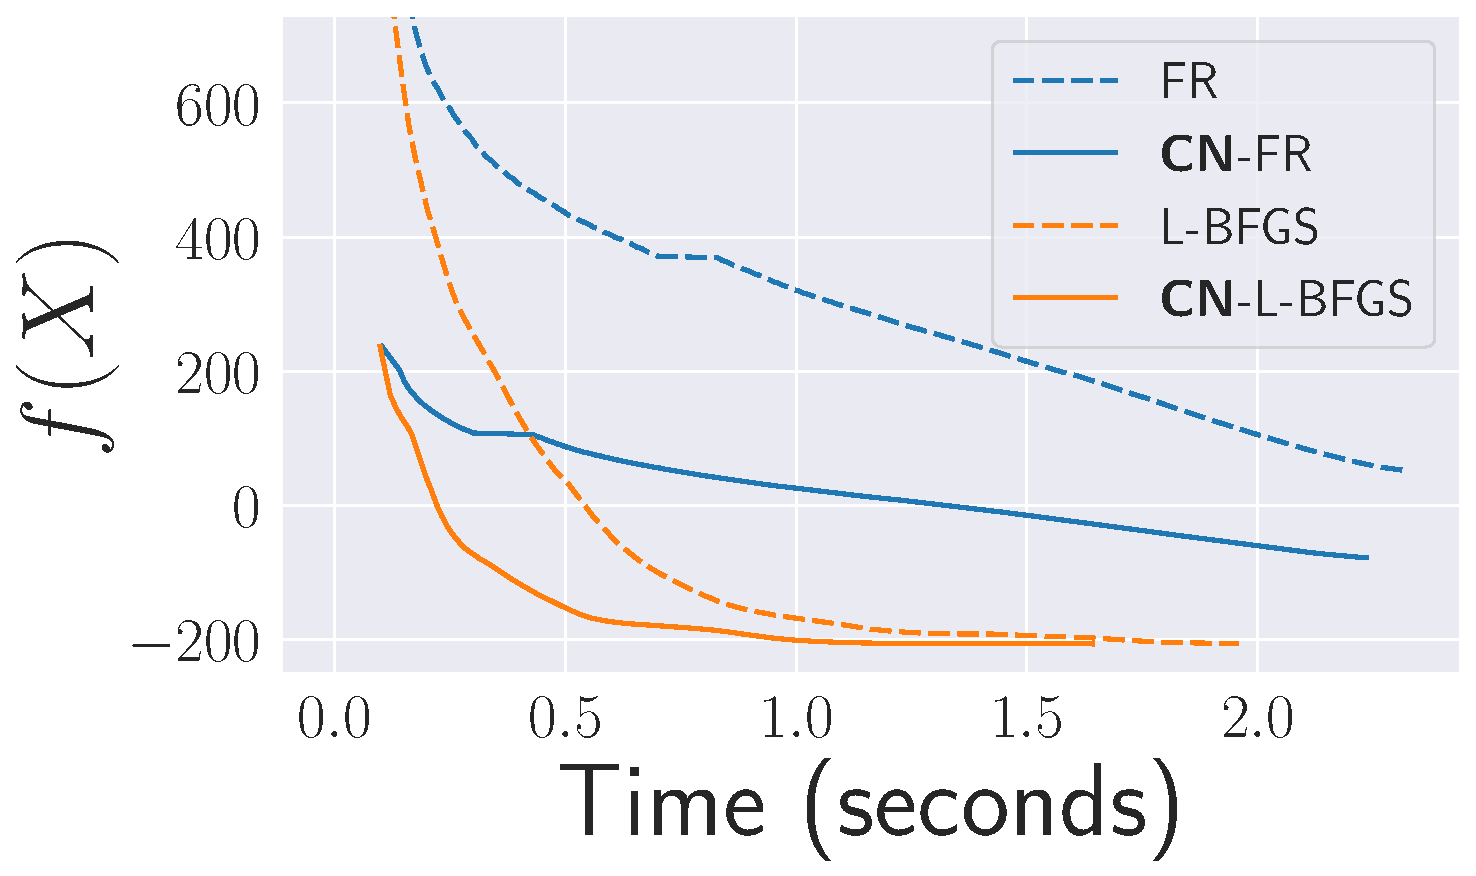
\includegraphics[width=0.275\columnwidth]{../main/individual/plot/jagmesh1.pdf}} &
        \makecell{\small{\textsf{FR}}                                                                                                                       \\[-0.2em]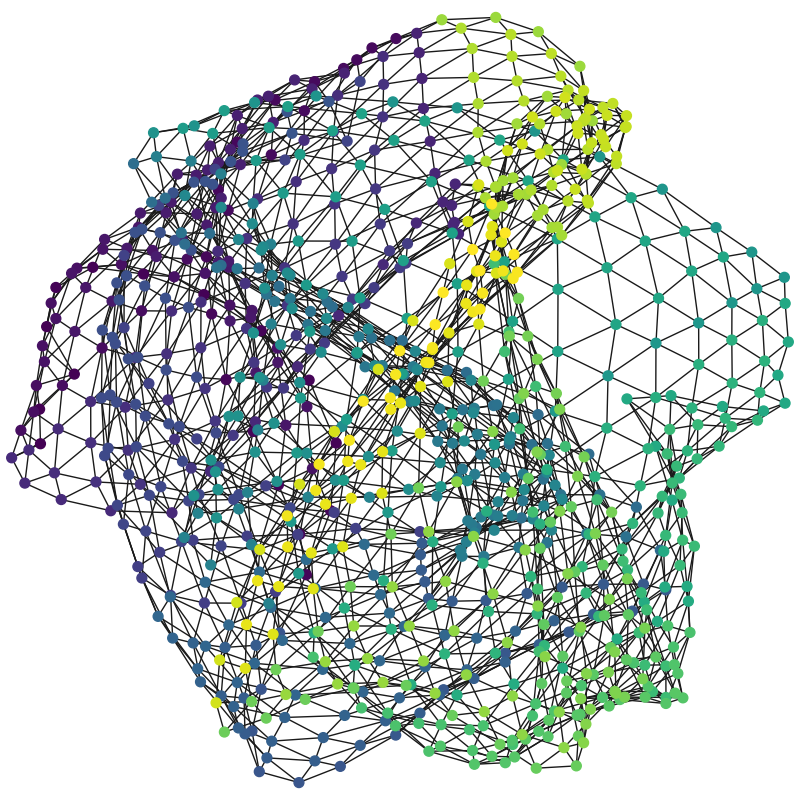
\includegraphics[width=0.135\columnwidth]{../main/individual/vis/jagmesh1_FR.png}} &
        \makecell{\small{\textsf{L-BFGS}}                                                                                                                   \\[-0.2em]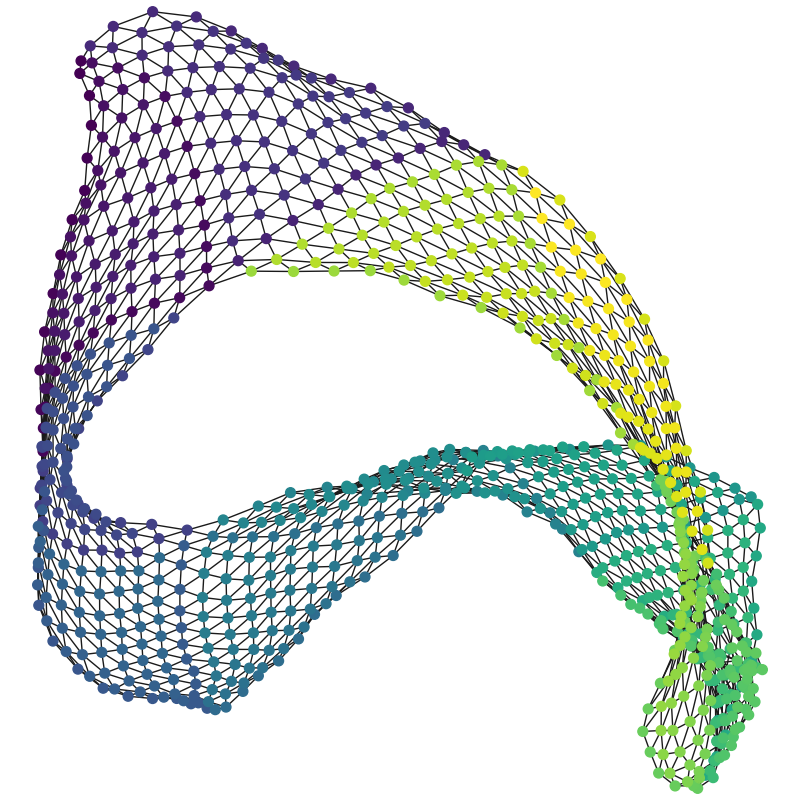
\includegraphics[width=0.135\columnwidth]{../main/individual/vis/jagmesh1_L-BFGS.png}} &
        \makecell{\small{\textsf{\textbf{CN}-FR}}                                                                                                           \\[-0.2em]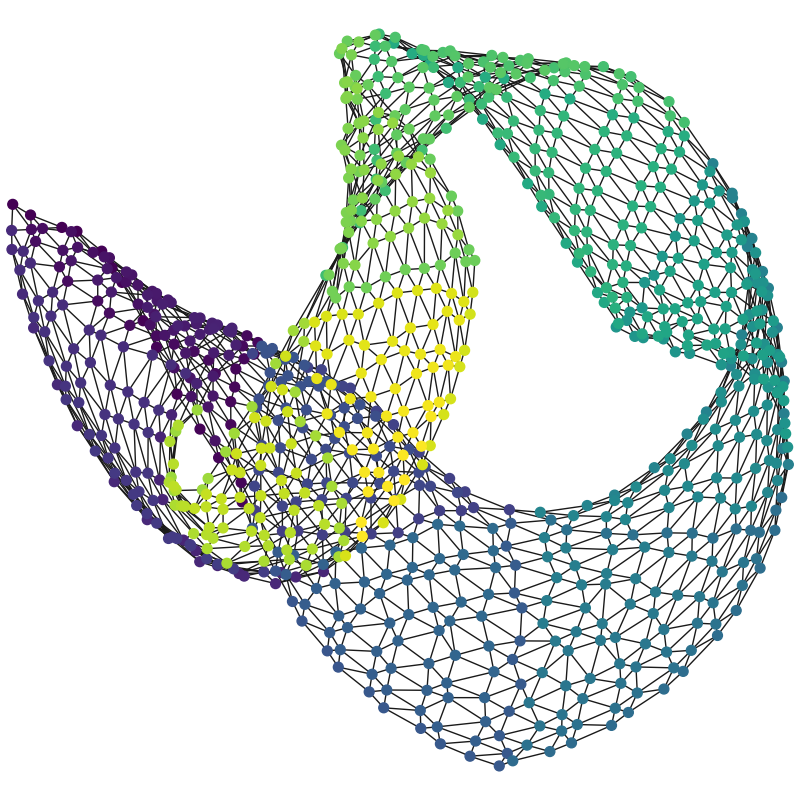
\includegraphics[width=0.135\columnwidth]{../main/individual/vis/jagmesh1_CN-FR.png}} &
        \makecell{\small{\textsf{\textbf{CN}-L-BFGS}}                                                                                                       \\[-0.2em]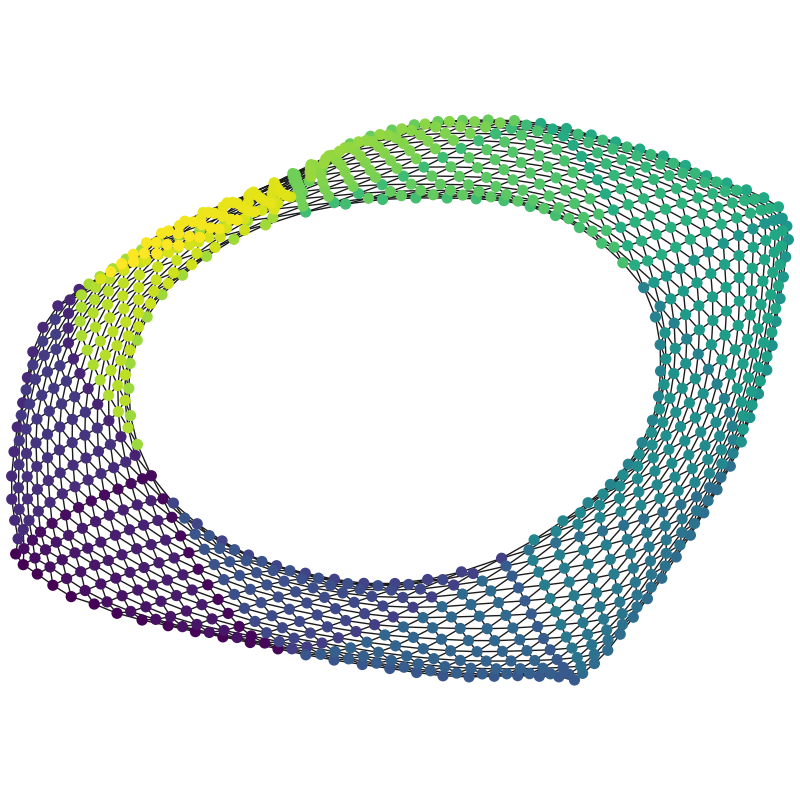
\includegraphics[width=0.135\columnwidth]{../main/individual/vis/jagmesh1_CN-L-BFGS.png}} &
        \makecell{\small{\textsf{BEST}}                                                                                                                     \\[-0.2em]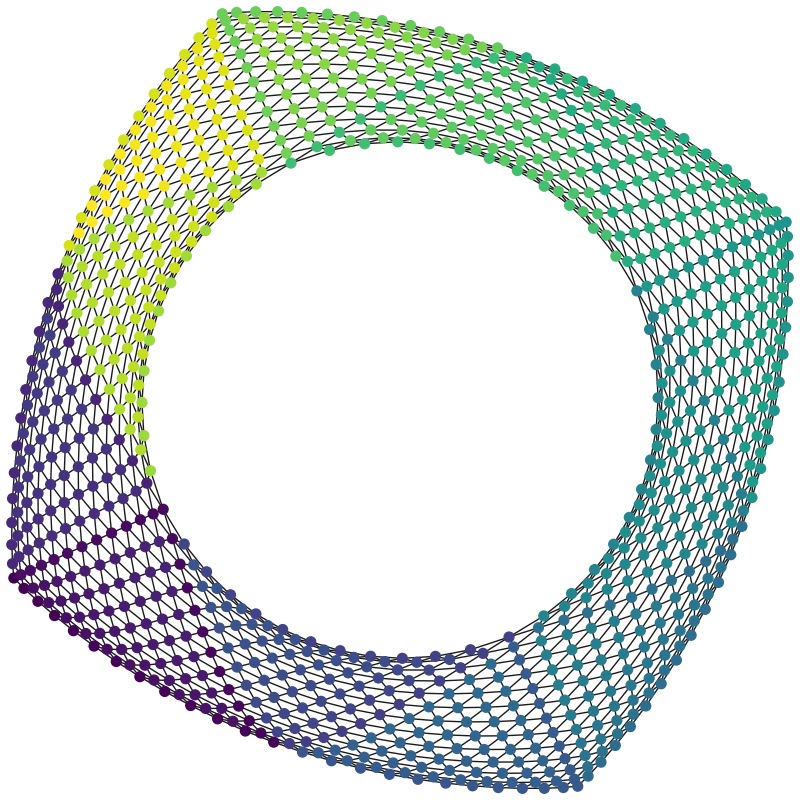
\includegraphics[width=0.135\columnwidth]{../main/individual/vis/opt_jagmesh1.png}} \\

        \multicolumn{6}{c}{\textbf{\texttt{dwt\_1005}} $(\abs{V}=1005, \abs{E}=3808, \text{sparsity}=0.755\text{\%})$ \quad Figures are at 100 iterations.} \\
        \raisebox{-.5\height}{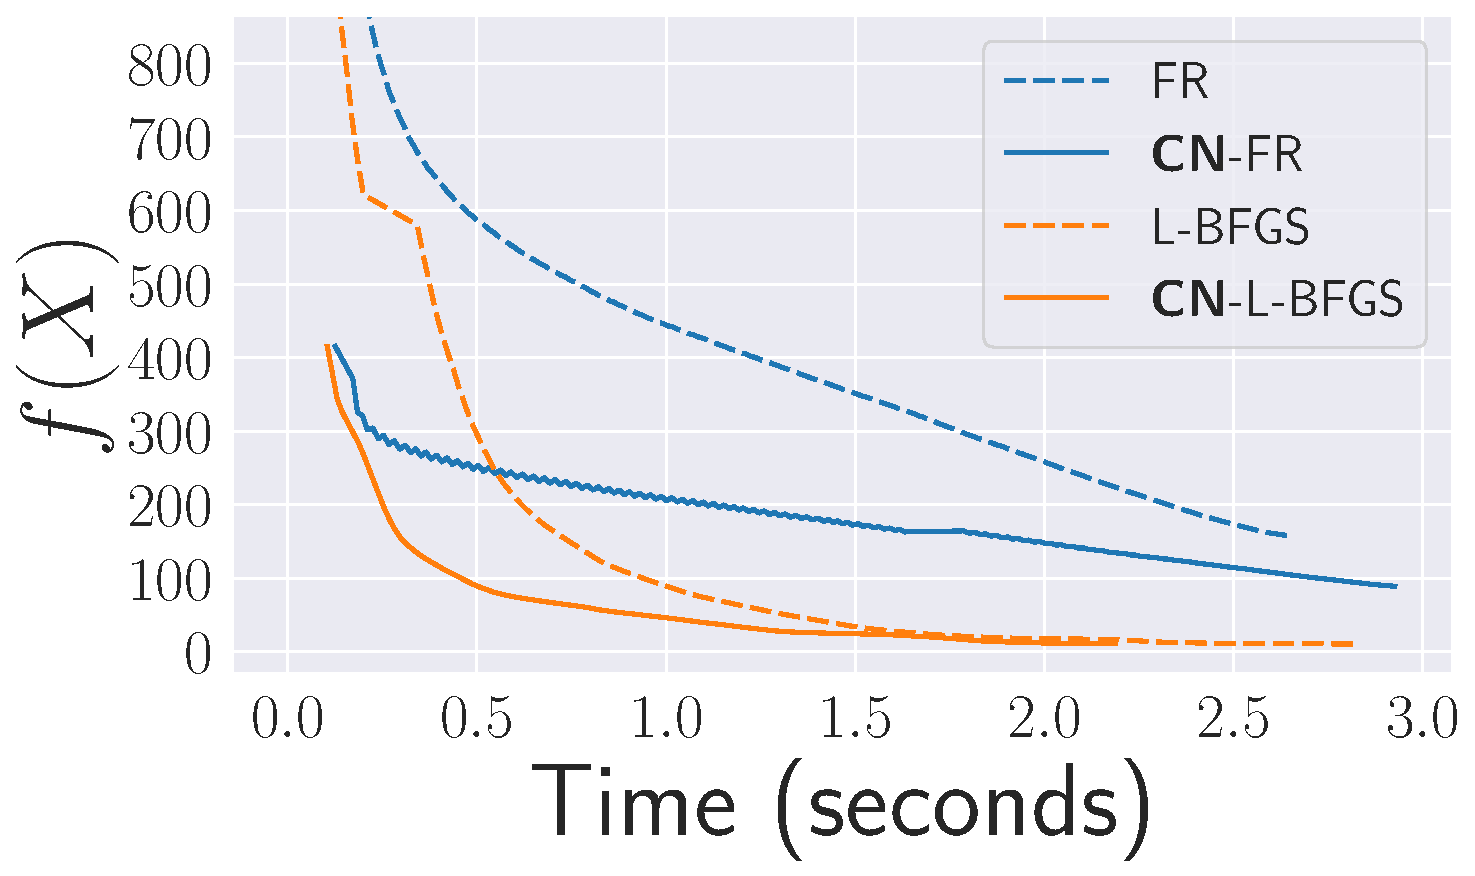
\includegraphics[width=0.275\columnwidth]{../main/individual/plot/dwt_1005.pdf}} &
        \makecell{\small{\textsf{FR}}                                                                                                                       \\[-0.2em]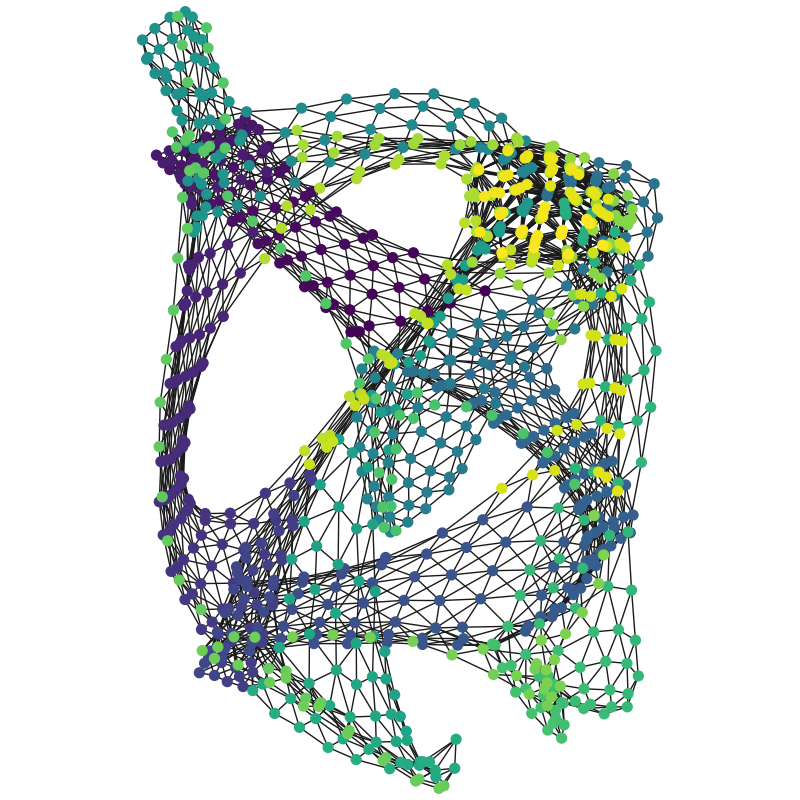
\includegraphics[width=0.135\columnwidth]{../main/individual/vis/dwt_1005_FR.png}} &
        \makecell{\small{\textsf{L-BFGS}}                                                                                                                   \\[-0.2em]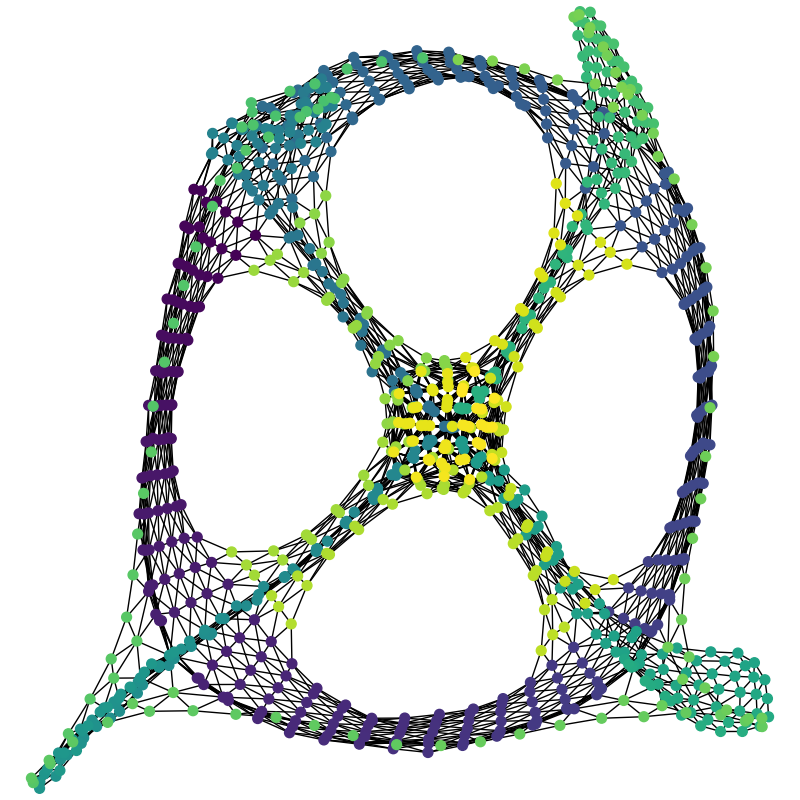
\includegraphics[width=0.135\columnwidth]{../main/individual/vis/dwt_1005_L-BFGS.png}} &
        \makecell{\small{\textsf{\textbf{CN}-FR}}                                                                                                           \\[-0.2em]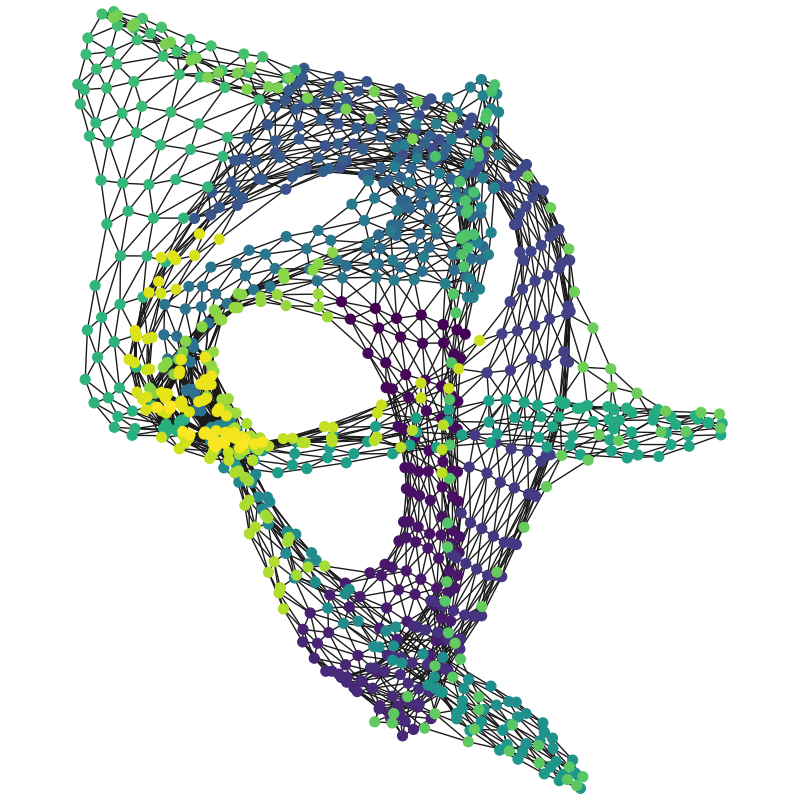
\includegraphics[width=0.135\columnwidth]{../main/individual/vis/dwt_1005_CN-FR.png}} &
        \makecell{\small{\textsf{\textbf{CN}-L-BFGS}}                                                                                                       \\[-0.2em]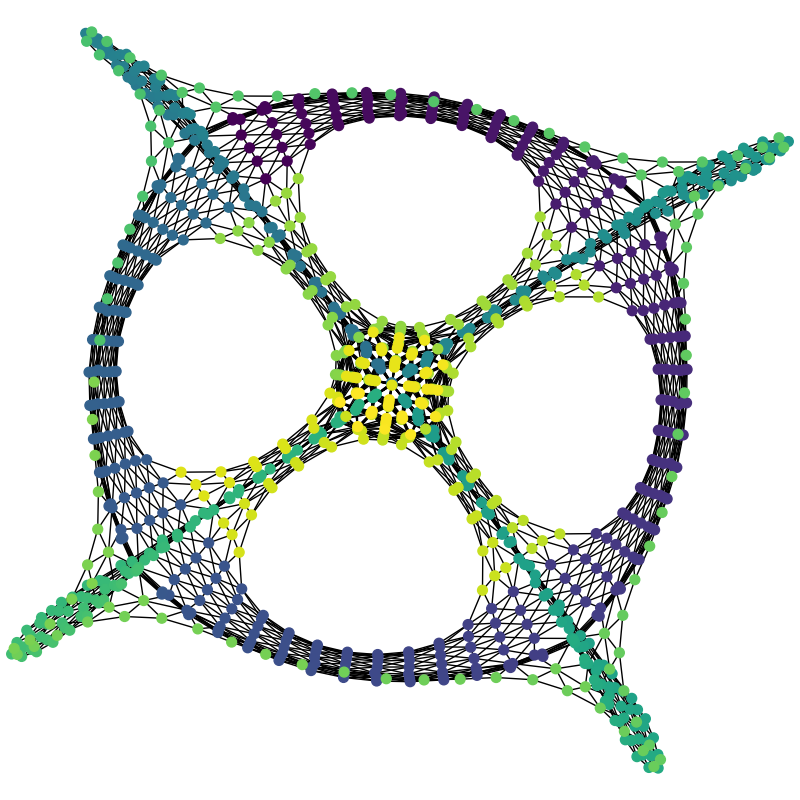
\includegraphics[width=0.135\columnwidth]{../main/individual/vis/dwt_1005_CN-L-BFGS.png}} &
        \makecell{\small{\textsf{BEST}}                                                                                                                     \\[-0.2em]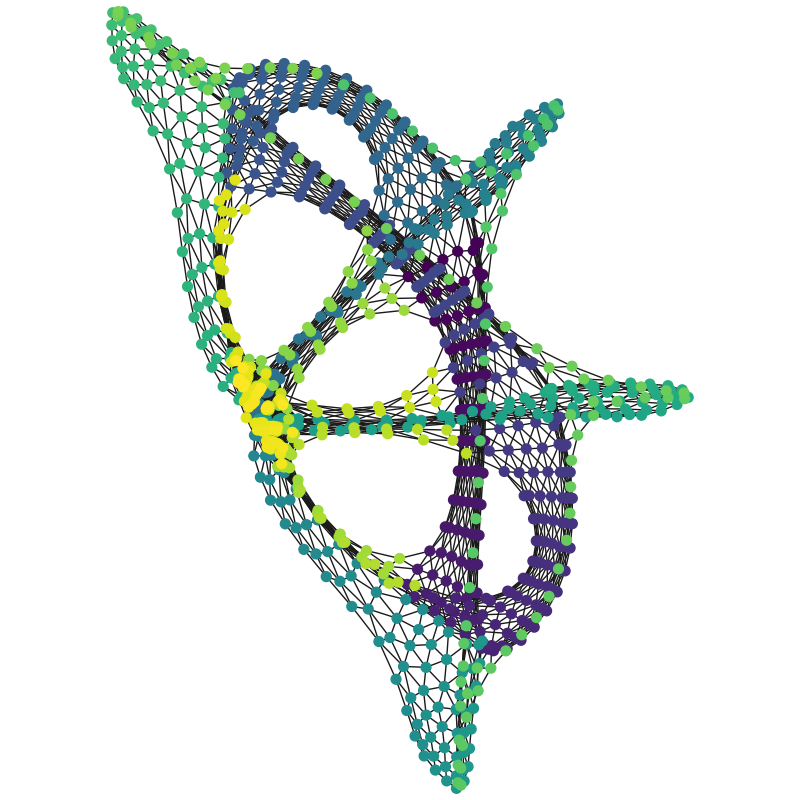
\includegraphics[width=0.135\columnwidth]{../main/individual/vis/opt_dwt_1005.png}} \\
      \end{tabular}
      \caption{``BEST''は提案手法の500反復目の状態}
    \end{figure}
  \end{frame}
\fi

\ifShowHidden
  \begin{frame}{実験結果 2/2}
    \begin{figure}[h]
      \centering
      \addtolength{\tabcolsep}{-0.5em}
      \begin{tabular}{cccccc}
        \multicolumn{6}{c}{\textbf{\texttt{dwt\_2680}} $(\abs{V}=2680, \abs{E}=11173, \text{sparsity}=0.311\text{\%})$ \quad Figures are at 150 iterations.} \\
        \raisebox{-.5\height}{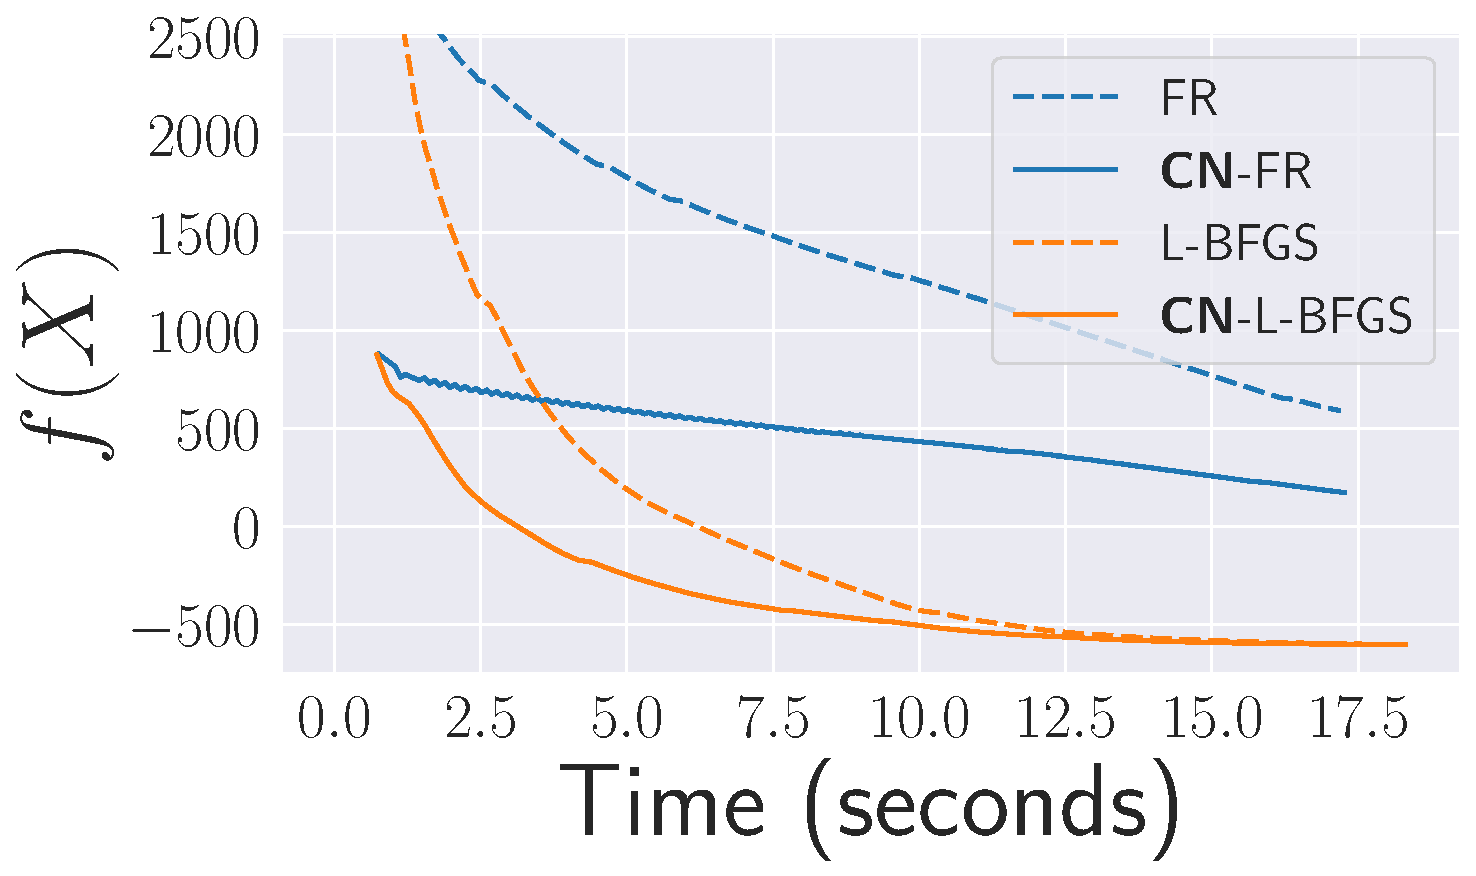
\includegraphics[width=0.275\columnwidth]{../main/individual/plot/dwt_2680.pdf}} &
        \makecell{\small{\textsf{FR}}                                                                                                                        \\[-0.2em]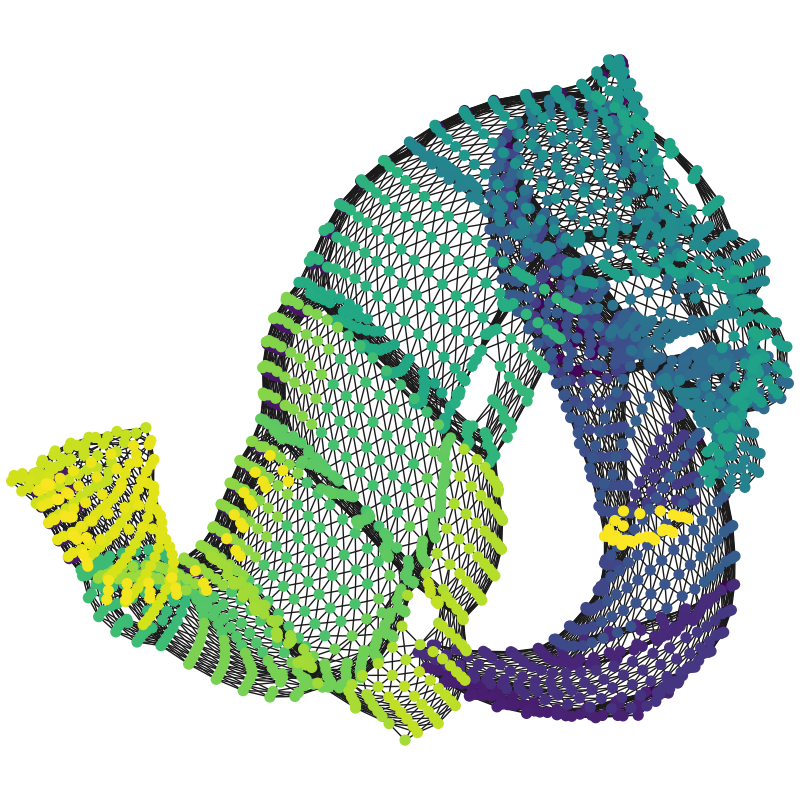
\includegraphics[width=0.135\columnwidth]{../main/individual/vis/dwt_2680_FR.png}} &
        \makecell{\small{\textsf{L-BFGS}}                                                                                                                    \\[-0.2em]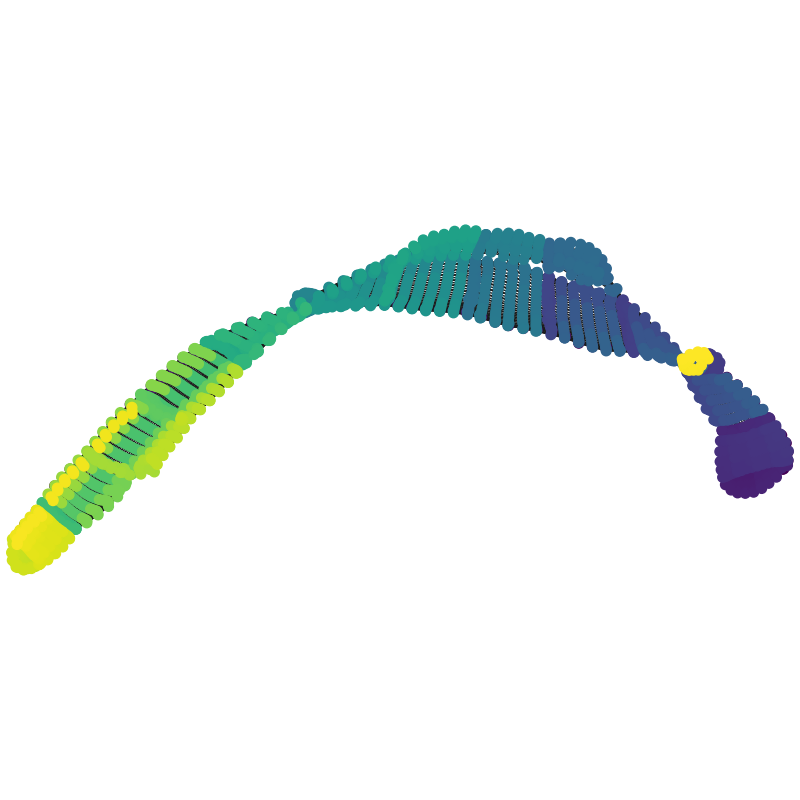
\includegraphics[width=0.135\columnwidth]{../main/individual/vis/dwt_2680_L-BFGS.png}} &
        \makecell{\small{\textsf{\textbf{CN}-FR}}                                                                                                            \\[-0.2em]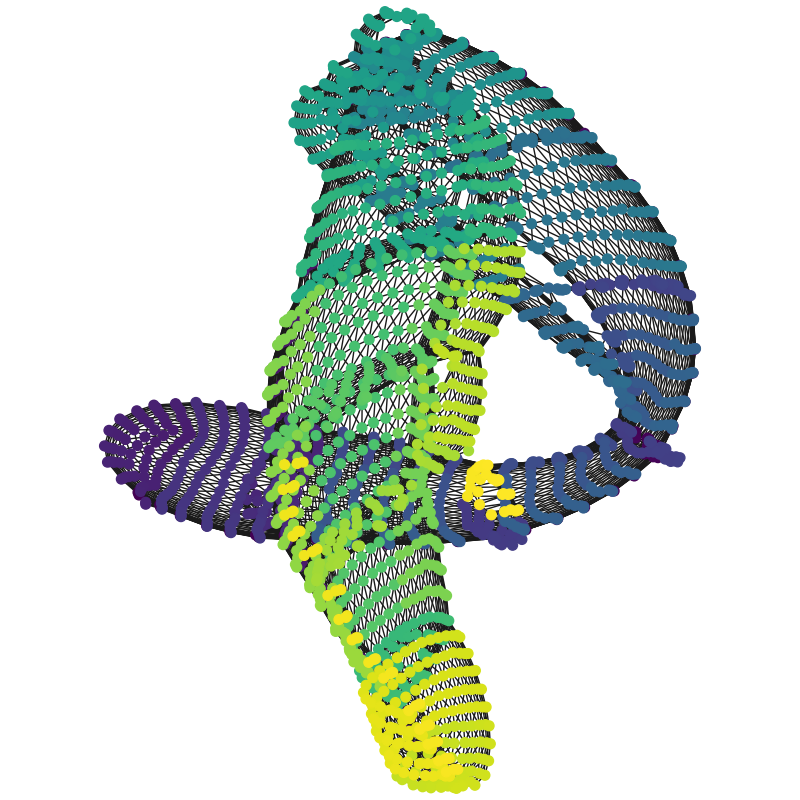
\includegraphics[width=0.135\columnwidth]{../main/individual/vis/dwt_2680_CN-FR.png}} &
        \makecell{\small{\textsf{\textbf{CN}-L-BFGS}}                                                                                                        \\[-0.2em]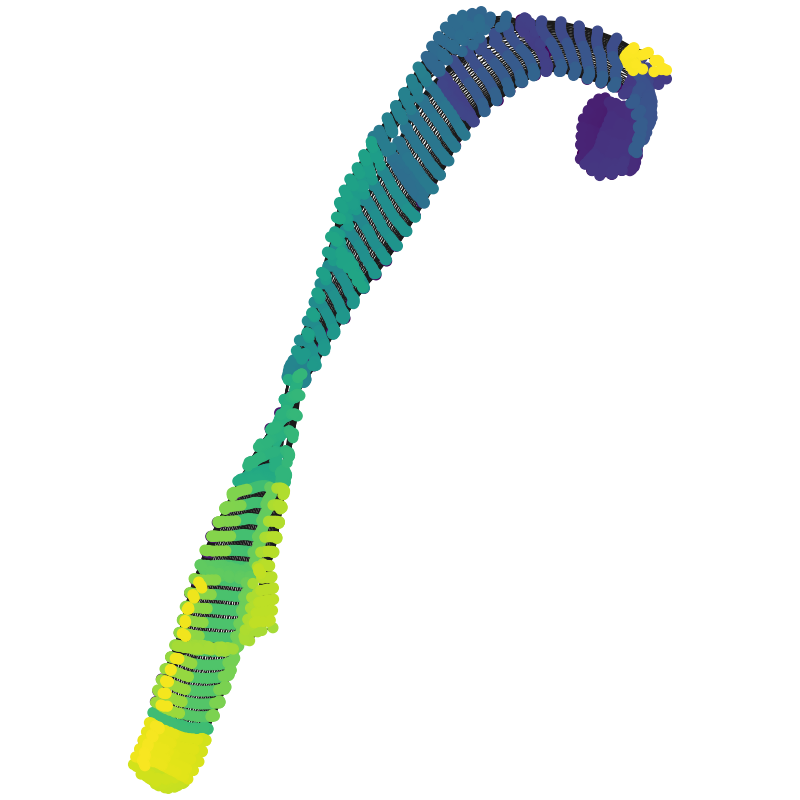
\includegraphics[width=0.135\columnwidth]{../main/individual/vis/dwt_2680_CN-L-BFGS.png}} &
        \makecell{\small{\textsf{BEST}}                                                                                                                      \\[-0.2em]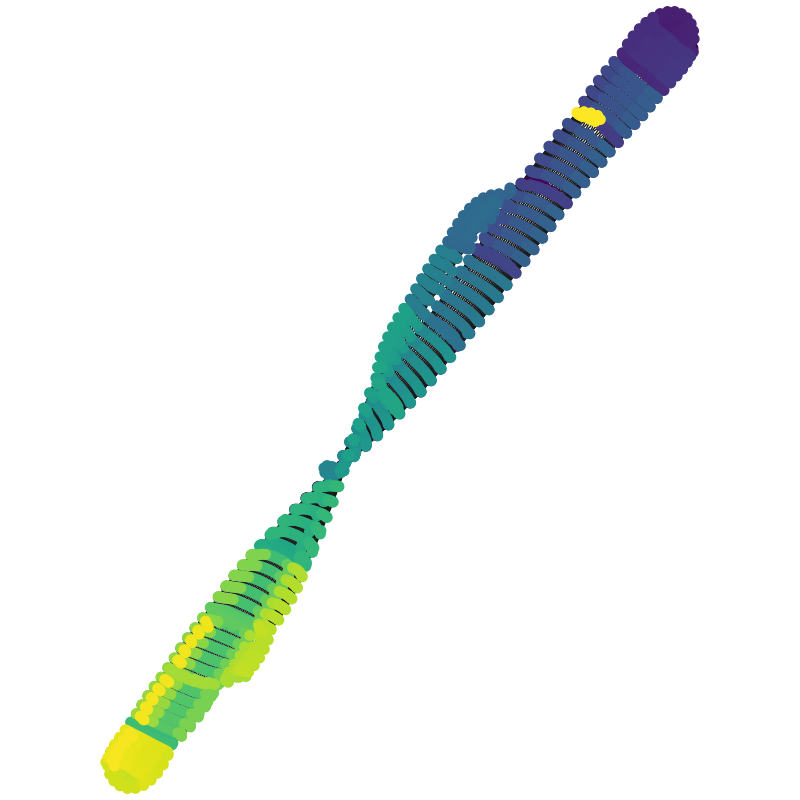
\includegraphics[width=0.135\columnwidth]{../main/individual/vis/opt_dwt_2680.png}} \\

        \multicolumn{6}{c}{\textbf{\texttt{3elt}} $(\abs{V}=4720, \abs{E}=13722, \text{sparsity}=0.123\text{\%})$ \quad Figures are at 150 iterations.}      \\
        \raisebox{-.5\height}{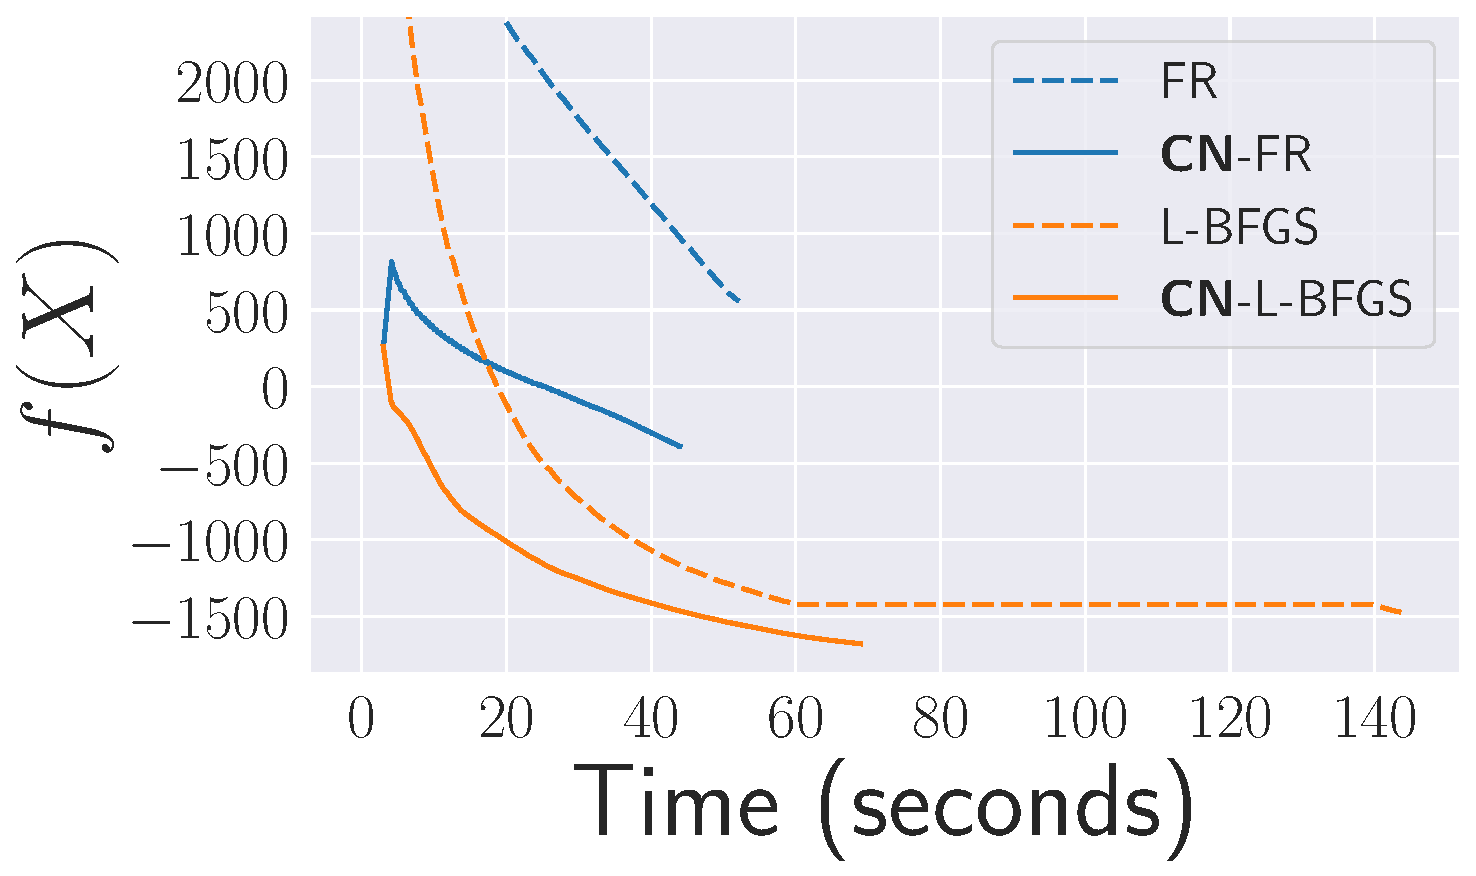
\includegraphics[width=0.275\columnwidth]{../main/individual/plot/3elt.pdf}}     &
        \makecell{\small{\textsf{FR}}                                                                                                                        \\[-0.2em]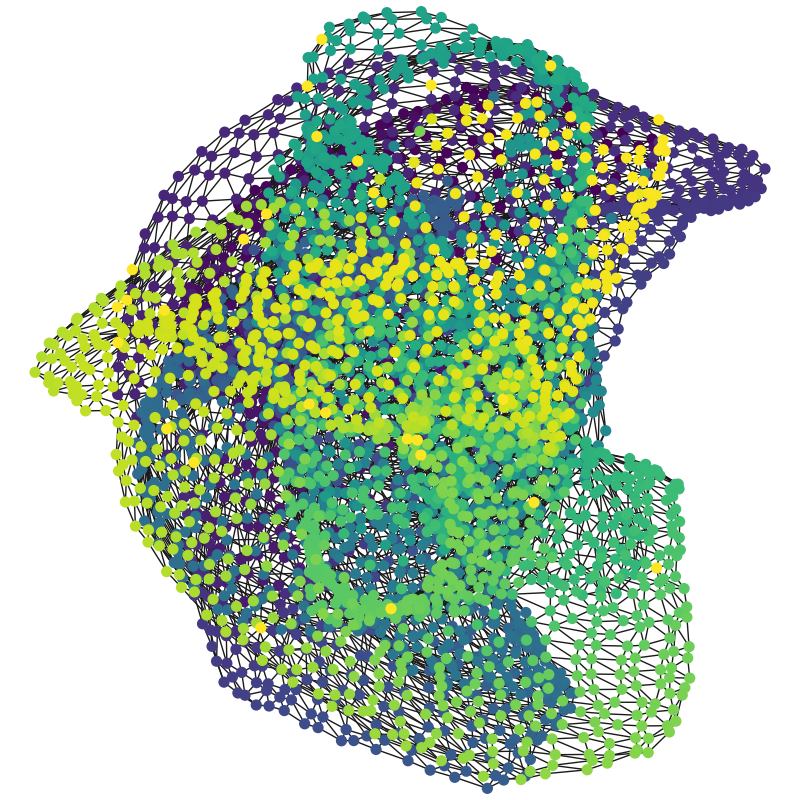
\includegraphics[width=0.135\columnwidth]{../main/individual/vis/3elt_FR.png}} &
        \makecell{\small{\textsf{L-BFGS}}                                                                                                                    \\[-0.2em]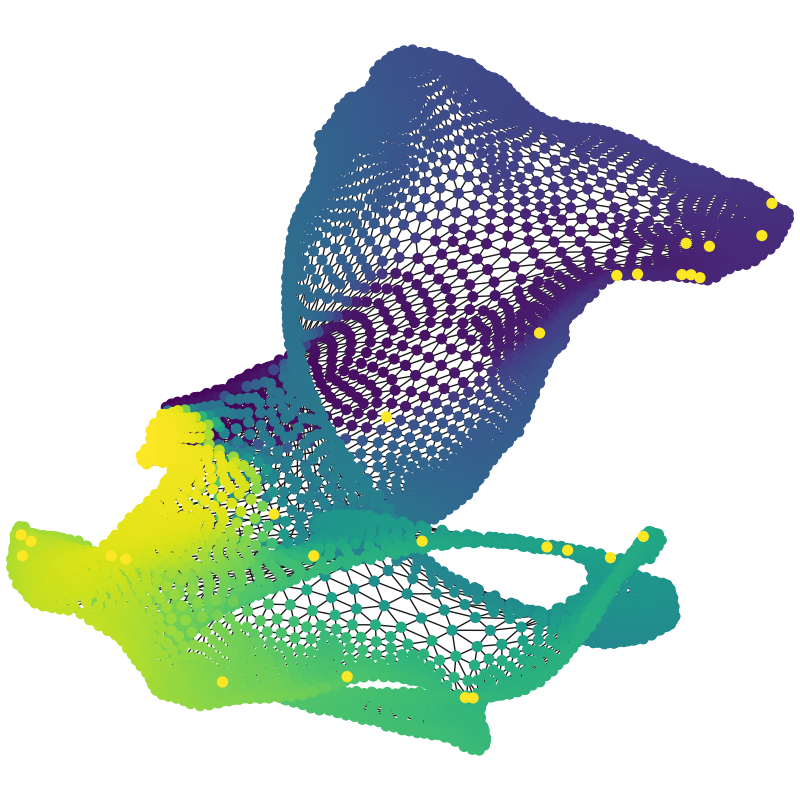
\includegraphics[width=0.135\columnwidth]{../main/individual/vis/3elt_L-BFGS.png}} &
        \makecell{\small{\textsf{\textbf{CN}-FR}}                                                                                                            \\[-0.2em]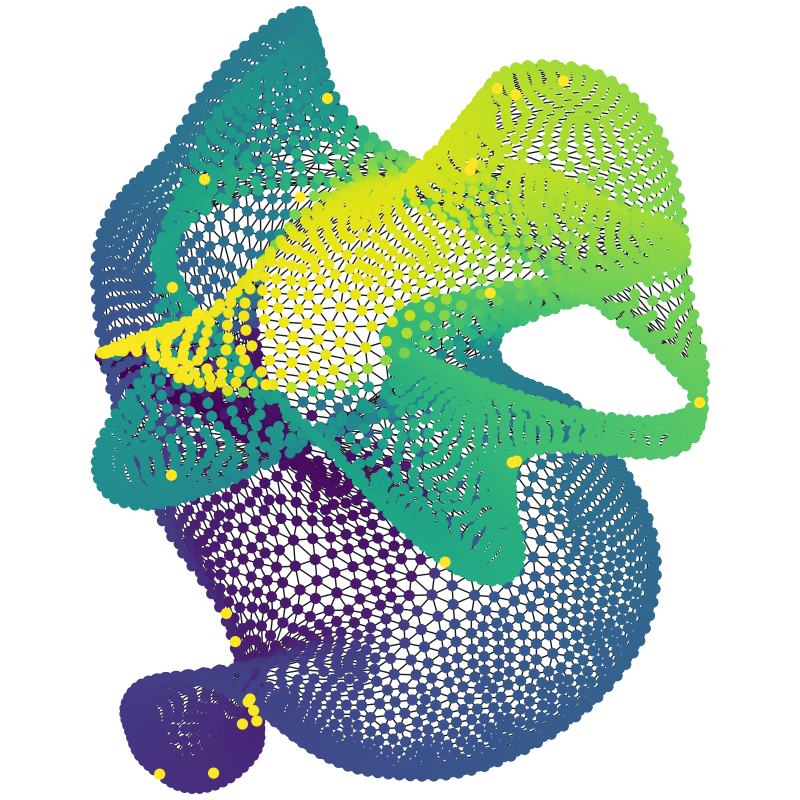
\includegraphics[width=0.135\columnwidth]{../main/individual/vis/3elt_CN-FR.png}} &
        \makecell{\small{\textsf{\textbf{CN}-L-BFGS}}                                                                                                        \\[-0.2em]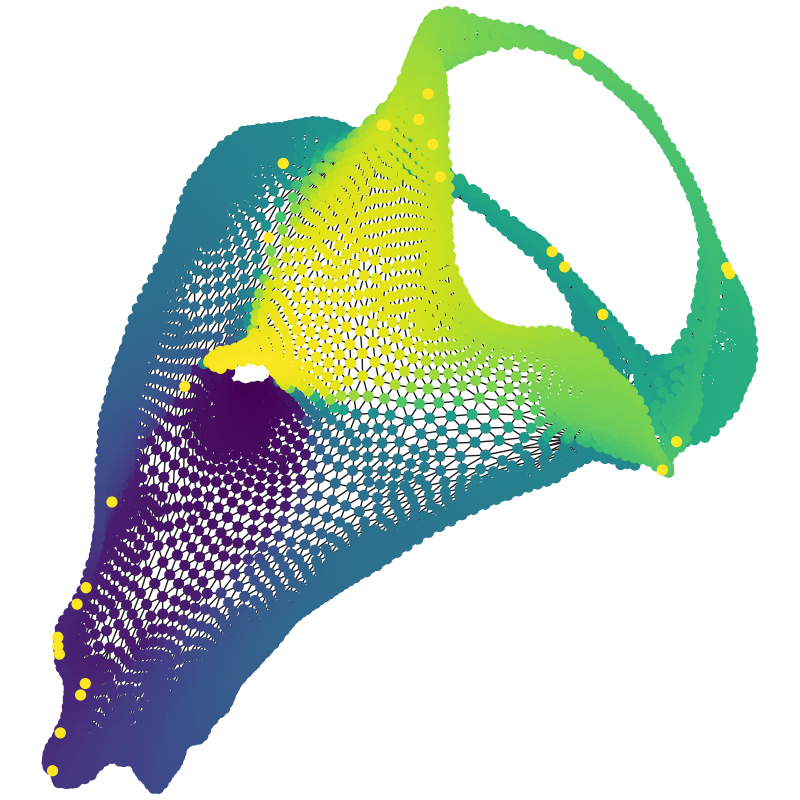
\includegraphics[width=0.135\columnwidth]{../main/individual/vis/3elt_CN-L-BFGS.png}} &
        \makecell{\small{\textsf{BEST}}                                                                                                                      \\[-0.2em]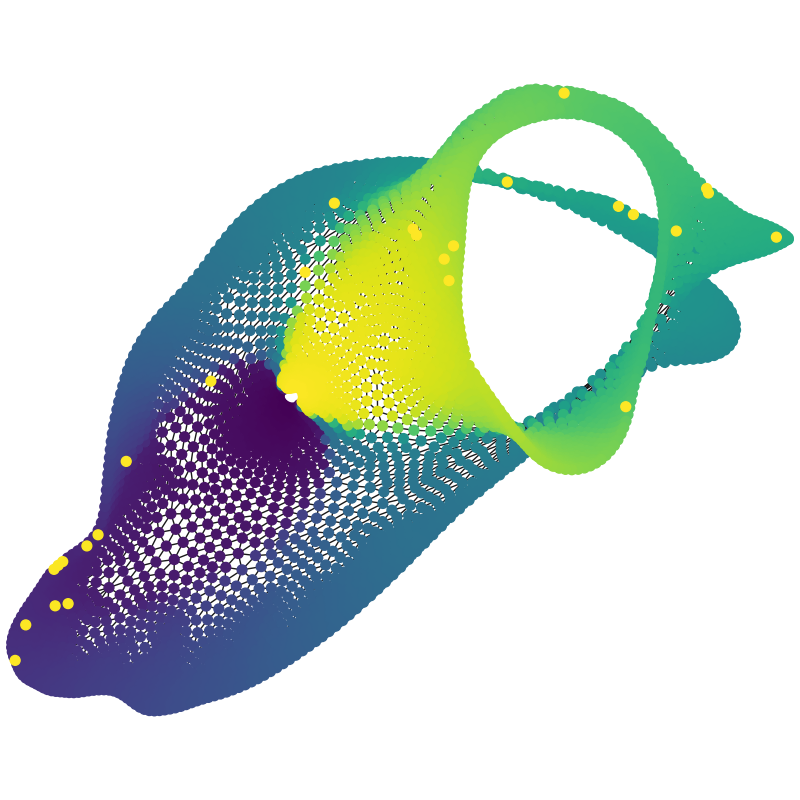
\includegraphics[width=0.135\columnwidth]{../main/individual/vis/opt_3elt.png}} \\
      \end{tabular}
      \caption{``BEST''は提案手法の500反復目の状態}
    \end{figure}
  \end{frame}
\fi

\ifShowHidden
  \begin{frame}{最後に}
    \vspace{-1em}
    \begin{figure}[htbp]
      \centering
      
\includegraphics[width=0.3\columnwidth]{QR_networkx.png}
    \end{figure}
    \vspace{-1em}
    \begin{block}{まとめと今後の展望}
      \begin{itemize}
        \item[\textbullet] 貢献1: 上記QR \quad 貢献2: 座標ニュートン方向を用いた初期配置の提案
        \item[\textbullet] Multilevel Approachと最適化手法の融合
        \item[\textbullet] グラフ同型判定問題は、2つのグラフの直和を対称に描画するのと似た問題
        \item[\textbullet] より広く、L-BFGS法自体を更に改善させることは出来ないか? (現在の我々の研究)
      \end{itemize}
    \end{block}
  \end{frame}
\fi

\setbeamercolor{structure}{fg=blendedblue}
\setbeamercolor{block title}{fg=blendedblue!50!black}

\ifShowHidden
  \begin{frame}[allowframebreaks]{Reference}
    \beamertemplatetextbibitems
    \bibliographystyle{plainnat}
    \bibliography{../main/FruchtermanReingoldByRandomSubspace.bib}
    % \begin{thebibliography}{1}
    % \end{thebibliography}
  \end{frame}
\fi

\end{document}